\documentclass[preprint,12pt]{elsarticle}
\usepackage{graphicx}
\usepackage[margin=1.0in]{geometry}
\usepackage{color, colortbl}
\usepackage{hyperref}
\usepackage{float}
\usepackage{lineno}
\linenumbers
% \usepackage[affil-it]{authblk}
\usepackage{subcaption}
\newcommand{\note}[1]{\textcolor{blue}{#1}}
\definecolor{LightCyan}{rgb}{0.88,1,1}
\definecolor{LightRose}{rgb}{1,0.88,0.88}
\definecolor{LightGreen}{rgb}{0.88,1,0.88}

\title{Convolutional Auto-Encoders for Drift Chamber data de-noising for CLAS12}
\author[1]{Gagik Gavalian}
\author[2]{Polykarpos Thomadakis}
\author[2]{Angelos Angelopoulos}
\author[3]{Raffaella De Vita}
\author[2]{Nikos Chrisochoides}

%\author[1]{Veronique Ziegler}

\address[1]{Jefferson Lab, Newport News, VA, USA}
\address[2]{CRTC, Department of Computer Science, Old Dominion University, Norfolk, VA, USA}
\address[3]{INFN, Sezione di Genova, 16146 Genova, Italy}

\begin{document}

%\begin{titlepage}
\begin{abstract}
In this article we present results of using Convolutional Auto-Encoders for de-noising raw data for CLAS12 drift chambers.
The de-noising neural network provides increased efficiency in track reconstruction, also improved performance for high 
luminosity experimental data collection. The de-noising neural network used in conjunction with previously developed track 
classifier neural network~\cite{Gavalian:2022hfa} lead to significant track reconstruction efficiency increase for current luminosity
(incident beam current $45~nA$). The increase in experimentally measured quantities allow running experiments at more than 
twice higher luminosity (at $120~nA$) with same track reconstruction efficiency. This will lead to huge saving in accelerator 
operational costs, and large savings for Jefferson Lab and collaborating institutions.
\end{abstract}
%\end{titlepage}
\maketitle


\section{Introduction}

During past few years there was a big interest in using Artificial Intelligence (AI) in 
various ares of nuclear physics, from data processing to physics analysis. With continuously 
improving methods of Machine Learning (ML) and computational hardware it becomes easy to 
substitute some computational tasks with ML algorithms leading to smaller and computationally
more efficient code base. In this article we discuss implementation of Convolutional Auto-Encoders 
for de-noising data from CLAS12~\cite{Burkert:2020akg} tracking detectors (Drift 
Chambers~\cite{Mestayer:2020saf}). The de-nosing was used to analyze simulated data to measure
improvement on track reconstruction efficiency.


\section{CLAS12 Drift Chambers}

The Drift Chambers (DC), which are  part of the large detector system of CLAS12 located in the experimental 
Hall-B at Jefferson Lab. They are used for charged particle detection in the forward direction 
(covering polar angles $5-35^\circ$). The CLAS12 forward detector is built around a six-coil 
toroidal magnet which divides the active detection area into six azimuthal regions, called “sectors”. 
For each sector there are separate drift chambers installed consisting of 3 regions. Each region contains 
two super-layers, each of them containing 6 layers of wires.   Each layer of drift chamber 
consists of 112 signal wires making each region a matrix of 12x112. The raw signal from 
one sector makes a matrix of 36x112, that is analyzed independently from other sectors
to extract trajectories of charged particles from raw signals. 

 \begin{figure}[!h]
\begin{center}
 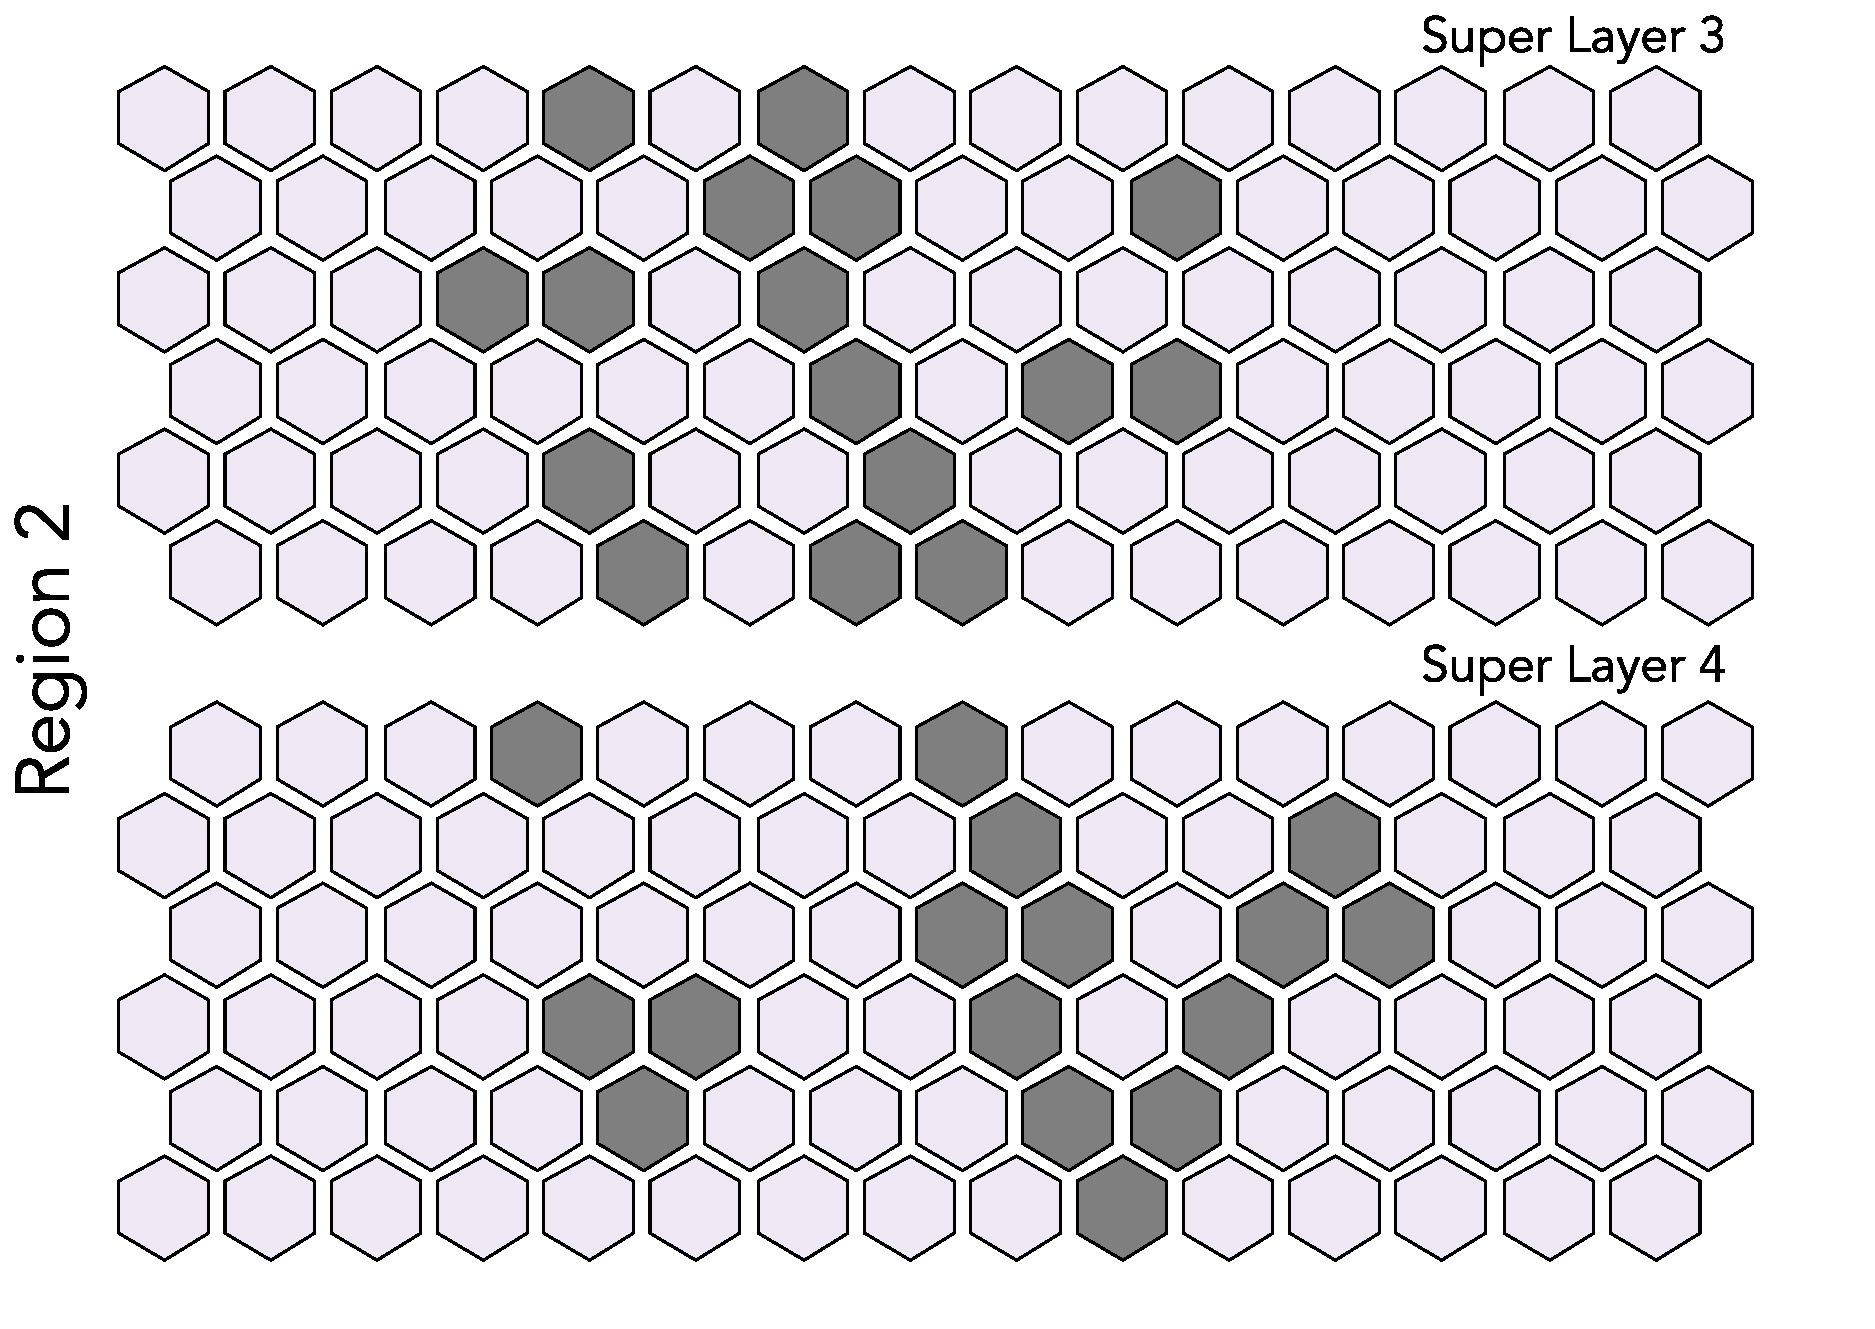
\includegraphics[width=3in]{images/dc_region_2_with_noise.pdf}
 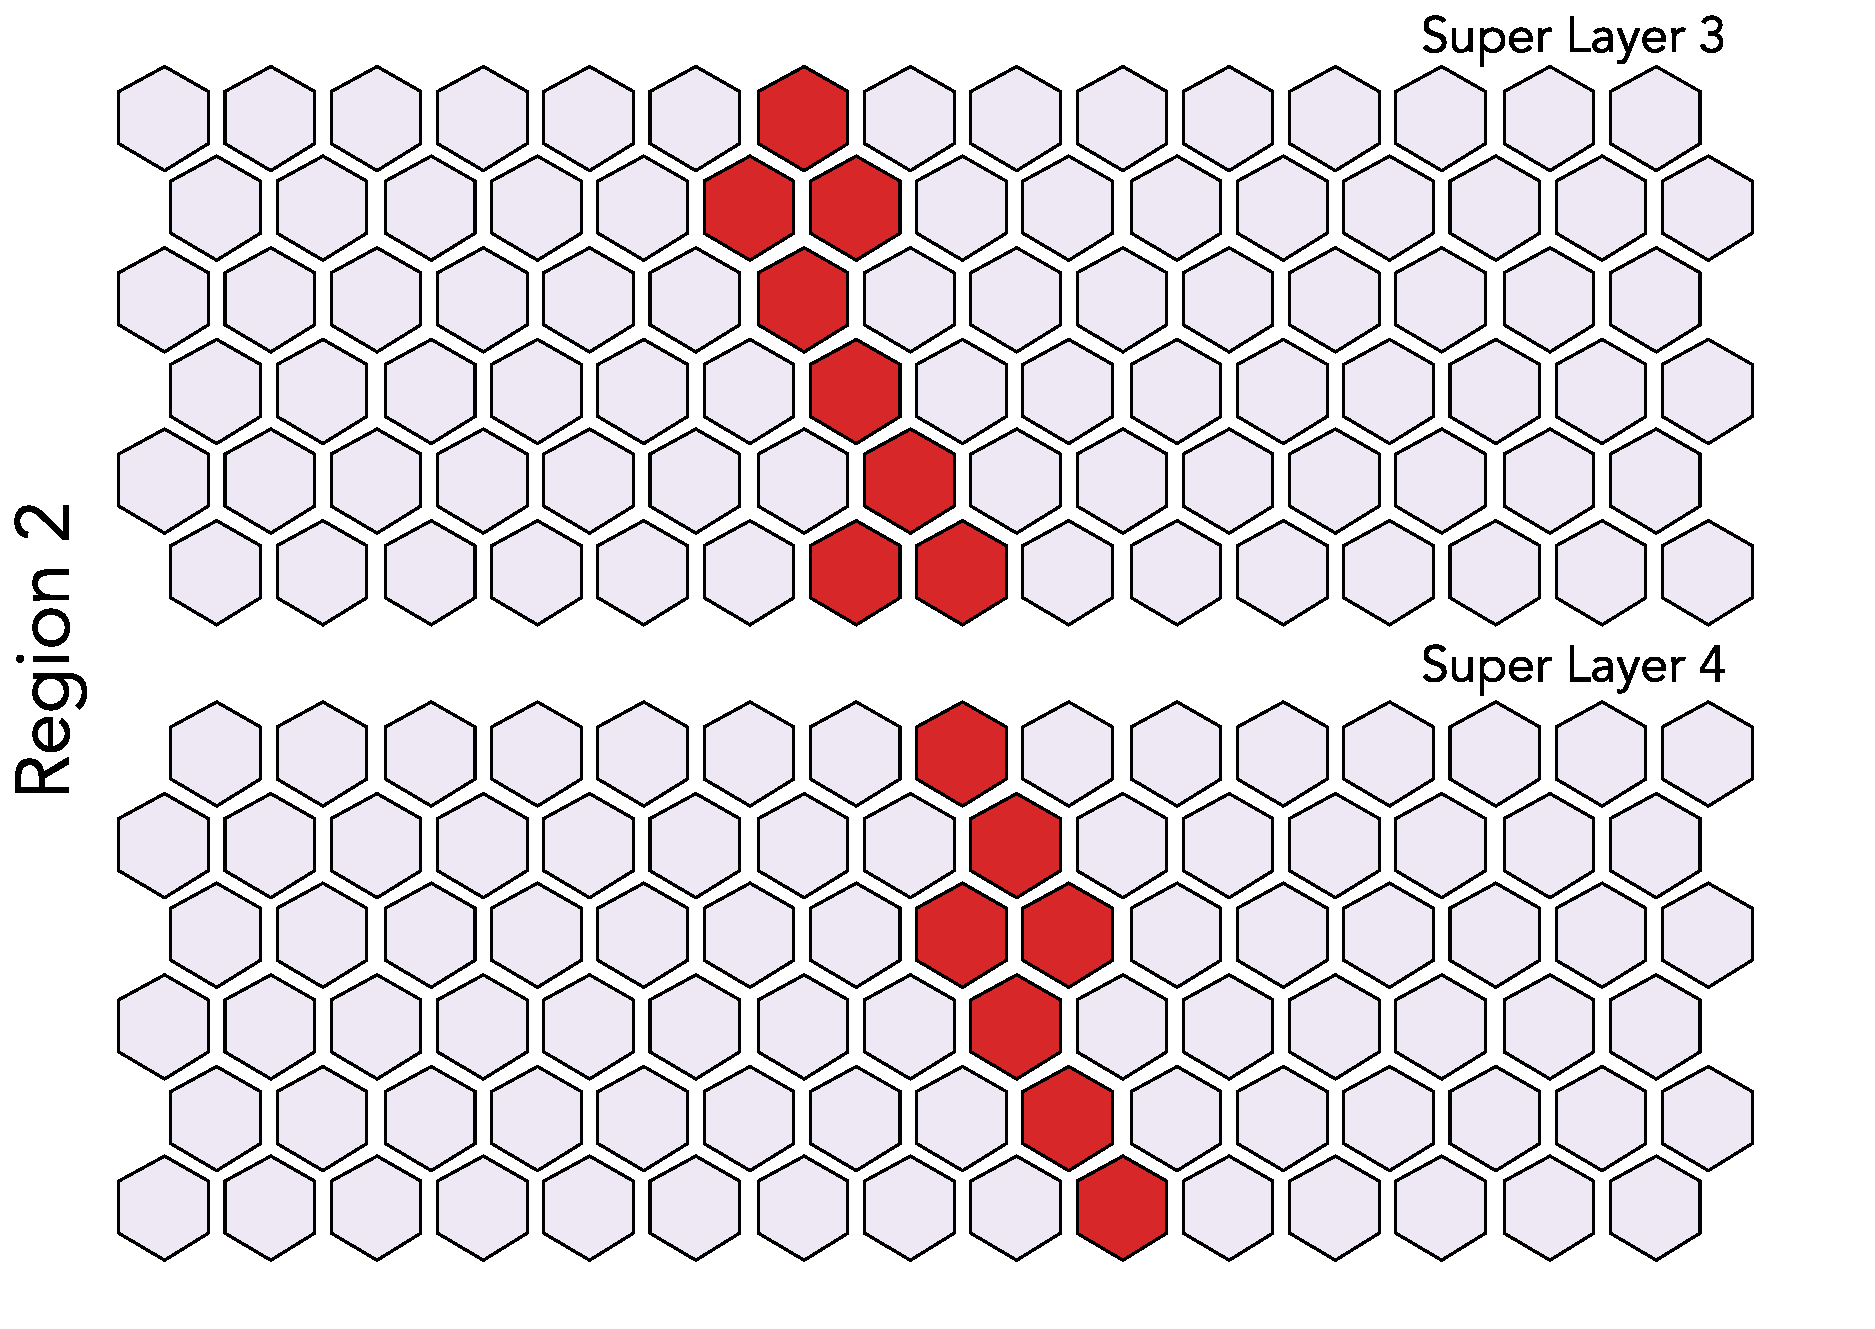
\includegraphics[width=3in]{images/dc_region_2_no_noise.pdf}
\caption {Example of clustering for one region of Drift Chambers. The left panel shows 
all the hits detected in the drift chamber (for this particular region), and the right panel 
shows results of clustering where some hits were identified as a background and were removed,
and the remaining hits were grouped to form a cluster.}
 \label{conv:denoising}
 \end{center}
\end{figure}

Each super-layer is analyzed separately for each sector and hits grouped together along the track trajectory 
are combined into clusters (or segments). In Figure~\ref{conv:denoising} the procedure is shown for one
region where the all hits (dark gray) are shown on the left panel, and clusters (red) are shown on the right panel,
by grouping neighboring wires after removing noise hits. Each super-layer
may have multiple clusters. The tracking algorithm creates a list of track candidates consisting of one cluster 
per super-layer and then analyzes the list to determine which candidates form a valid track. The identified 
tracks are further refined by passing them through Kalman filter~\cite{Kalman1960}. 
Examples of analyzed events in one sector can be seen in Figure~\ref{conv:trackfinding}, where 36x112 matrices
for four sectors are shown (not from the same event) with all signal hits in all layers (top row). The signal hits 
for clusters for identified tracks are shown on the bottom row. 


 \begin{figure}[!h]
\begin{center}
 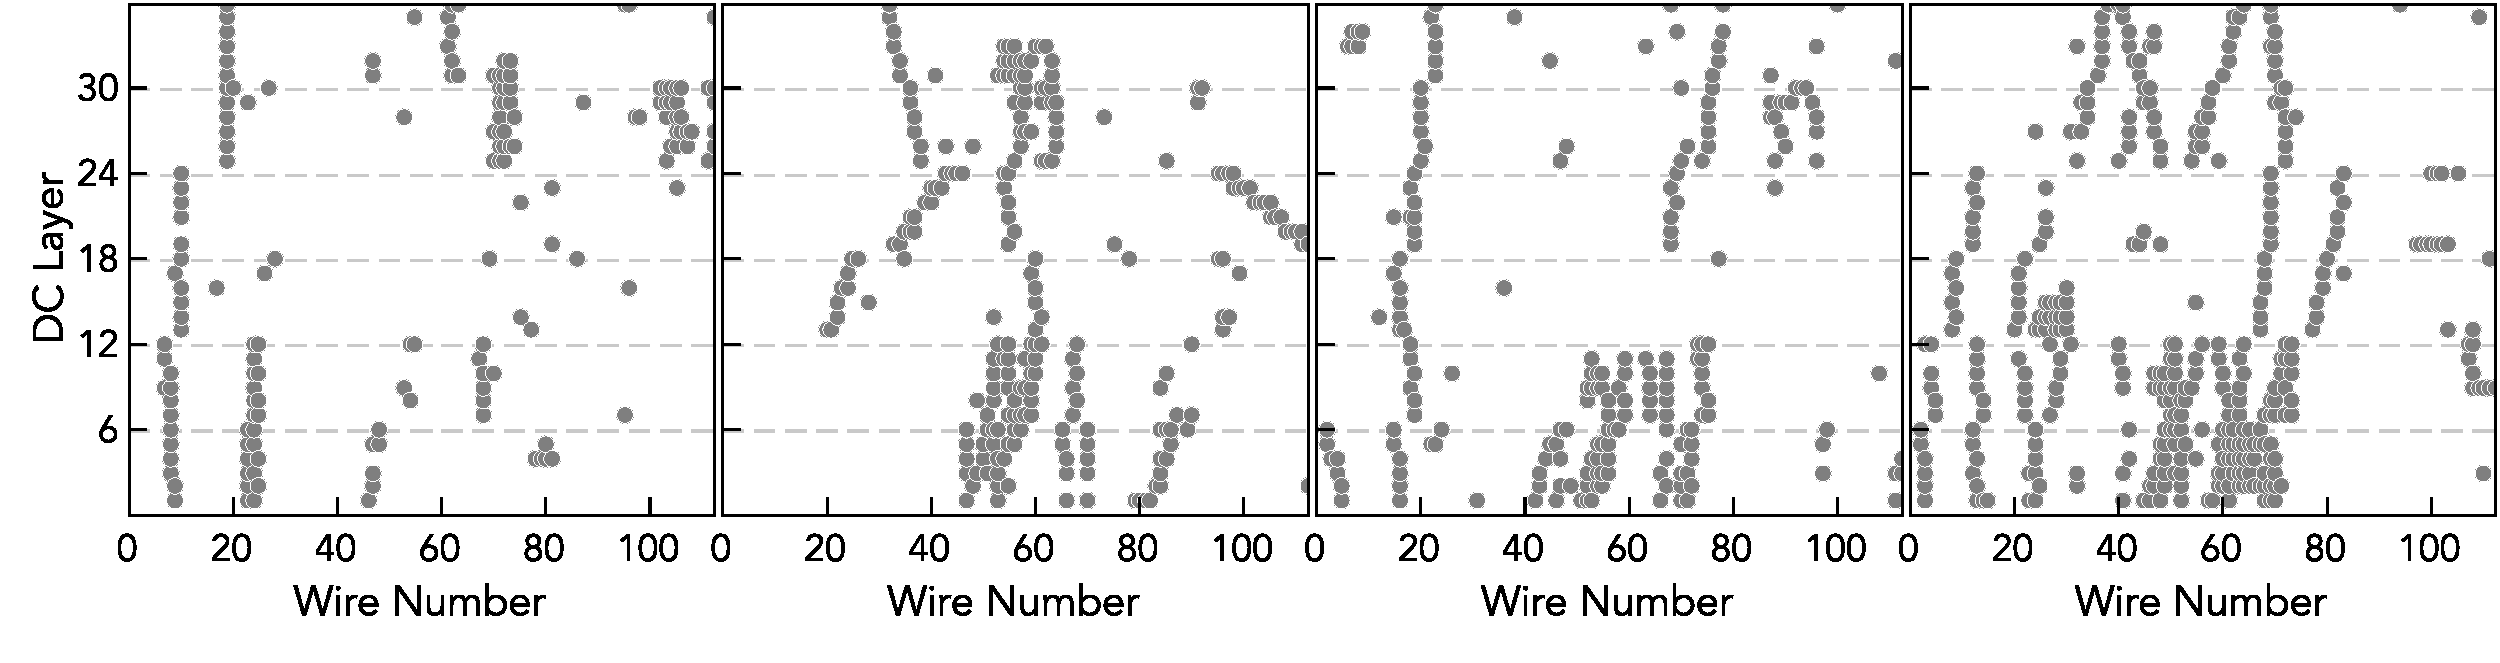
\includegraphics[width=6.0in]{images/dc_example_all_hits.pdf}
 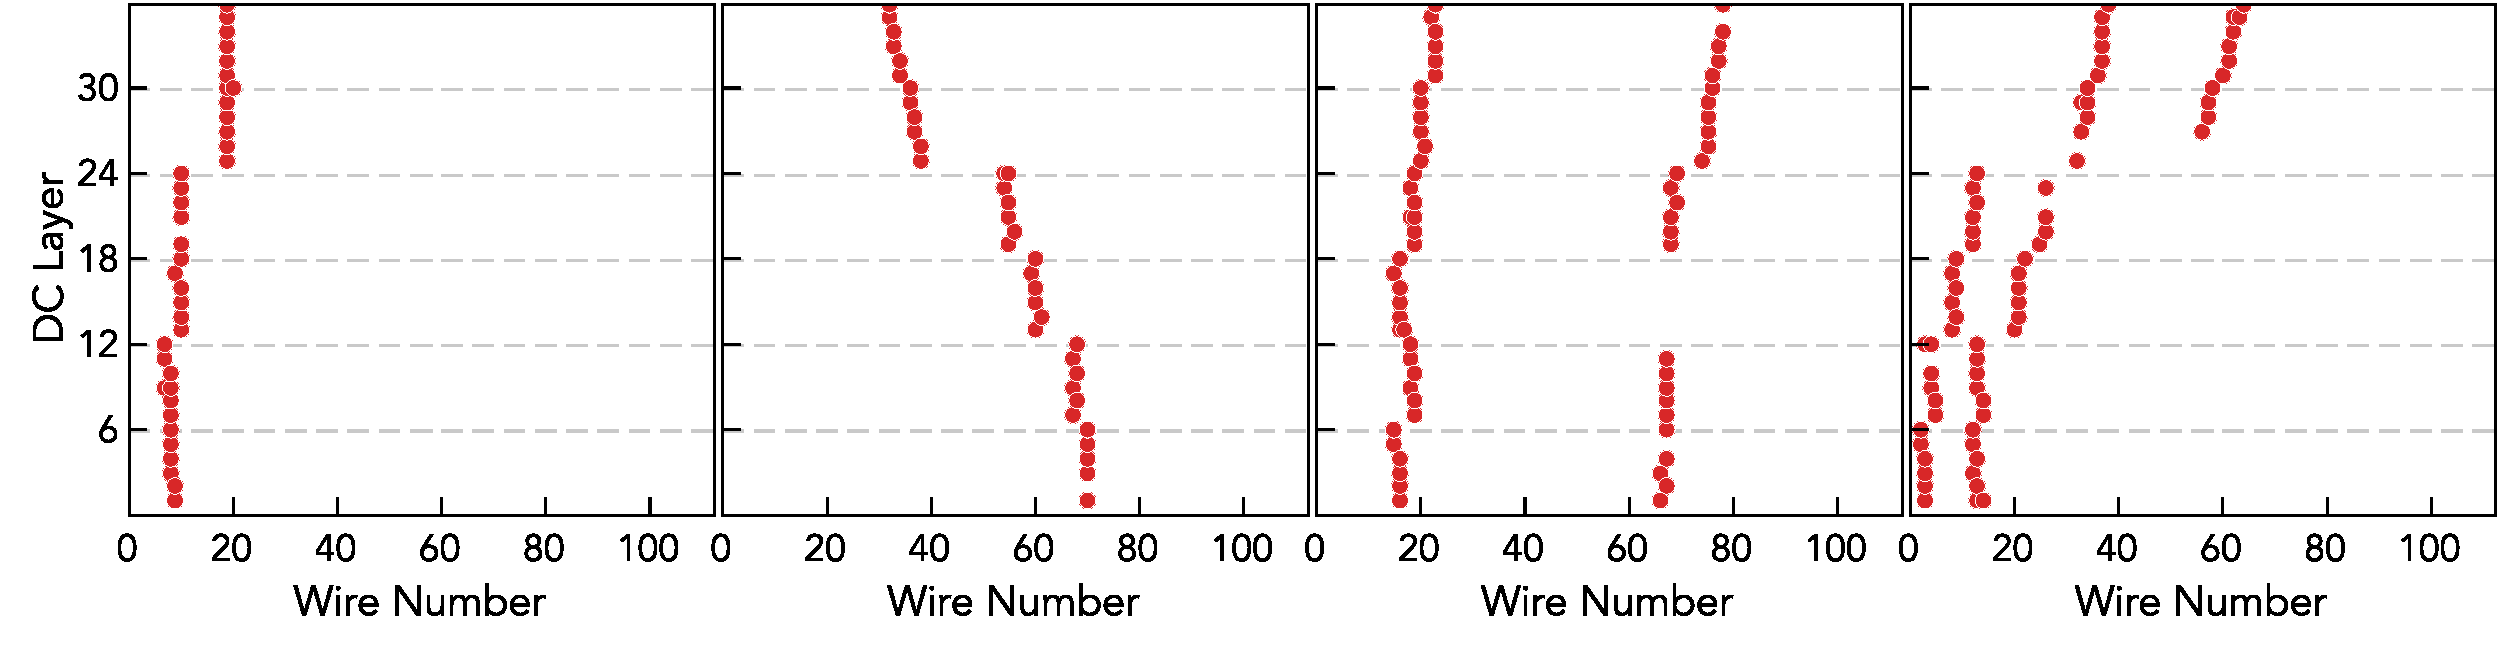
\includegraphics[width=6.0in]{images/dc_example_track_hits.pdf}
\caption {Example of reconstructed tracks in drift chambers. The signal hits in drift chambers are shown 
on the top row. The hits (clusters) belonging to identified tracks are shown on the bottom row. Dashed 
lines represent the boundaries of super-layers.}
 \label{conv:trackfinding}
 \end{center}
\end{figure}

As can be seen from the figure one or multiple tracks can be detected in one sector for the event. The efficiency
of finding these tracks depends on the cluster finding algorithm. With increased luminosity, the number of background 
hits increase, and it becomes difficult to separate background hits from signal hits due to heavy overlap between them.
This results in lost clusters and eventually in a decrease of track finding efficiency. 
In this work Machine Learning is used to remove background hits prior to clustering algorithm to improve cluster 
finding and consequentially track finding efficiency. The reconstructed experimental data is used to train Convolutional
Auto-Encoder for de-noising the drift chamber signal~\cite{Thomadakis:2022zcd}.



\section{Neural Network}

The Convolutional Auto-Encoder was used to de-noise raw data from CLAS12 drift chambers~\cite{Thomadakis:2022zcd}. The input and output for the network are matrices of size 36x112. The training data was extracted from experimental data. The raw hits (converted into a matrix) were used as an input for the neural network and a matrix constructed only from hits that belong to reconstructed tracks an output. In training data set multiple track hits were allowed in the output matrix. The structure of neural network can be seen on Figure~\ref{network:cnn_encoder}.

\begin{figure}[!h]
\begin{center}
 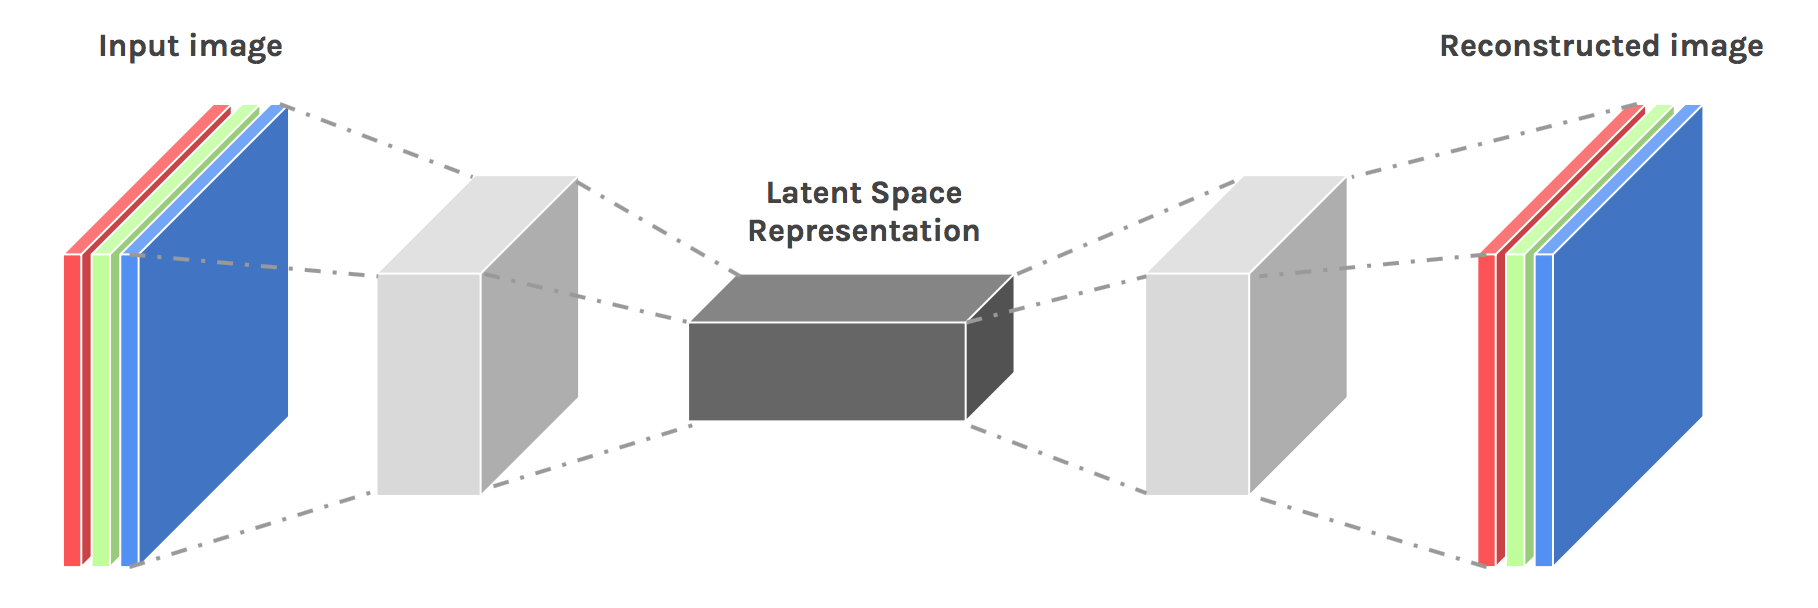
\includegraphics[width=5.1in]{images/convolutional-autoencoder.png}
\caption {De-noising neural network architecture.}
 \label{network:cnn_encoder}
 \end{center}
\end{figure}

For out implementation we used TensorFlow/Keras~\cite{keras-website} to train and evaluate the network. The resulting network parameters (weights) were saved in HDF5 file. The de-noiser implementation for CLAS12 reconstruction software is done using DeepLearning4J~\cite{dl4j-website} which supports model imports through HDF5 files. 


\section{Data Description}

\subsection{Monte-Carlo Simulation}

For these studies we used physics reactions generated using Pythia event generator and selected events were processed with GEMC (GEANT based detector simulation program) to produce data similar to experimental data. From generic Pythia output only events that contain four charged particle in as decay products in the final state (namely $e^-,\pi^+,\pi^-,p$) and any number of neutral particles. These events were used as an input to GEMC program that emulates CLAS12 detector responses and produces files with raw detector information.

Using these generated files new files were generated emulating different luminosity experimental conditions using CLAS12 standard background merging program \cite{Stepanyan:2020bg}. The background merging software uses real experimental data for given luminosity to extract background hits from all detector components that can later be overlayed on top of generated data to emulate high background running conditions. For our studies we used background files corresponding to $45~nA$, $50~nA$ and $55~nA$. Combining them sequentially we generated data corresponding to $45~nA$, $95~nA$ and $150~nA$. The $95~nA$ data sample was produced by merging $45~nA$ background file with the output of GEMC and then merging it with $50~nA$ background data. Similarly by merging $45~nA$, $50~nA$ and $55~nA$ in sequence we obtained data sample corresponding to $150~nA$. 

Most CLAS12 experiments run with $45~nA$ electron beam, and we want to measure performance impact of de-noising procedure for standard running conditions, and also see if we can run at higher beam currents (luminosity) which will potentially increase the statistical power of experiments.

\subsection{Data Analysis}

To study the effect of de-noising on particle reconstruction efficiency we processed produced data samples through stand-alone de-noiser program to produce de-noised counterparts of simulated data for each luminosity setting. The both data samples were processed using CLAS12 data reconstruction program. Then the track reconstruction efficiency was calculated for both data samples (original and de-noised) as a function of luminosity. The track reconstruction efficiency was calculated following standard (for CLAS12) procedure~\cite{Stepanyan:2020bg}. The efficiency for positive  tracks is defines as a ratio of 
events containing an electron and a positive  hadron ($N_{eh^+}$) to the number of inclusive events with an electron reconstructed ($N_{e}$). The efficiency of negative tracks is calculated similarly:

\begin{equation}
L_t^+ = \frac{N_{h^+e}}{N_e} , L_t^- = \frac{N_{h^-e}}{N_e} 
\label{eq::eff}
\end{equation}

Track reconstruction efficiencies were compared for regular and de-noised data samples for different luminosity settings.

\subsection{Artificial Intelligence Assisted Tracking}

The CLAS12 data reconstruction software already contains neural networks helping to identify track candidates from combinations of clusters reconstructed in each of the super-layers of drift chambers~\cite{Gavalian:2022mlp}.
This network already provides big improvement of tracking efficiency compared to traditional reconstruction algorithm. The impact on physics (depending on number of particles in the reaction) is $15\%-35\%$ increase in statistics. 
In the standard reconstruction software user can chose to use assistance from AI in identifying tracks or use purely the conventional algorithm to identify track candidates. In our studies we first investigated the improvement of de-noising algorithm by using the conventional algorithm to identify tracks. Then we extended these studies to include AI track identification when processing raw and de-noised data. By doing this we want to disentangle the performance improvements arising from de-noising from AI assistance. 


 


\section{Pseudo-data analysis with de-noising}

In this section, we compare results from the analysis of the background merged MC data sample with files that were de-noised prior to running through CLAS12 reconstruction software. The comparison is done for data samples with different luminosities (namely $45~nA$, $95~nA$, and $150~nA$ electron beam incident on a $5cm$ long liquid hydrogen target). The data for the raw sample and the de-noised sample is processed with the same settings of CLAS12 reconstruction software and the tracks reconstructed in each sample are analyzed.

\subsection{Luminosity dependence}

The track reconstruction efficiency is calculated according to Eqs.~(\ref{eq::eff}), (\ref{eq::eff2}) and (\ref{eq::eff3}) for positively and negatively charged particles. The results are shown in Figure~\ref{lscan::conv_dn}. The track reconstruction efficiency is an integrated quantity over the particle phase space. In our studies, we used a pre-selected simulation sample of three particles in the final state, which does not necessarily have angular and momentum dependence similar to experimental data and the efficiency dependence on beam current can reflect this. In these studies, we show a relative increase in efficiency when our methods are applied to simulated data.

\begin{figure}[!h]
\begin{center}
 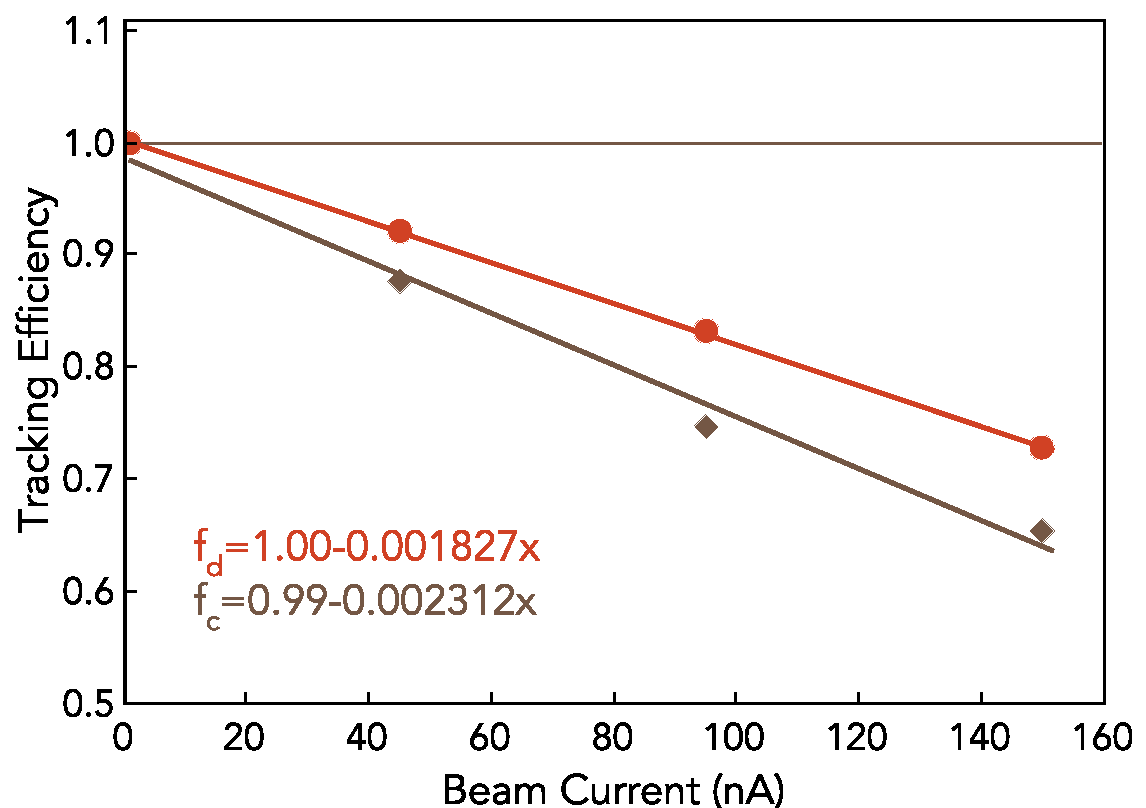
\includegraphics[width=3.1in]{images/figure_lscan_pos.pdf}
 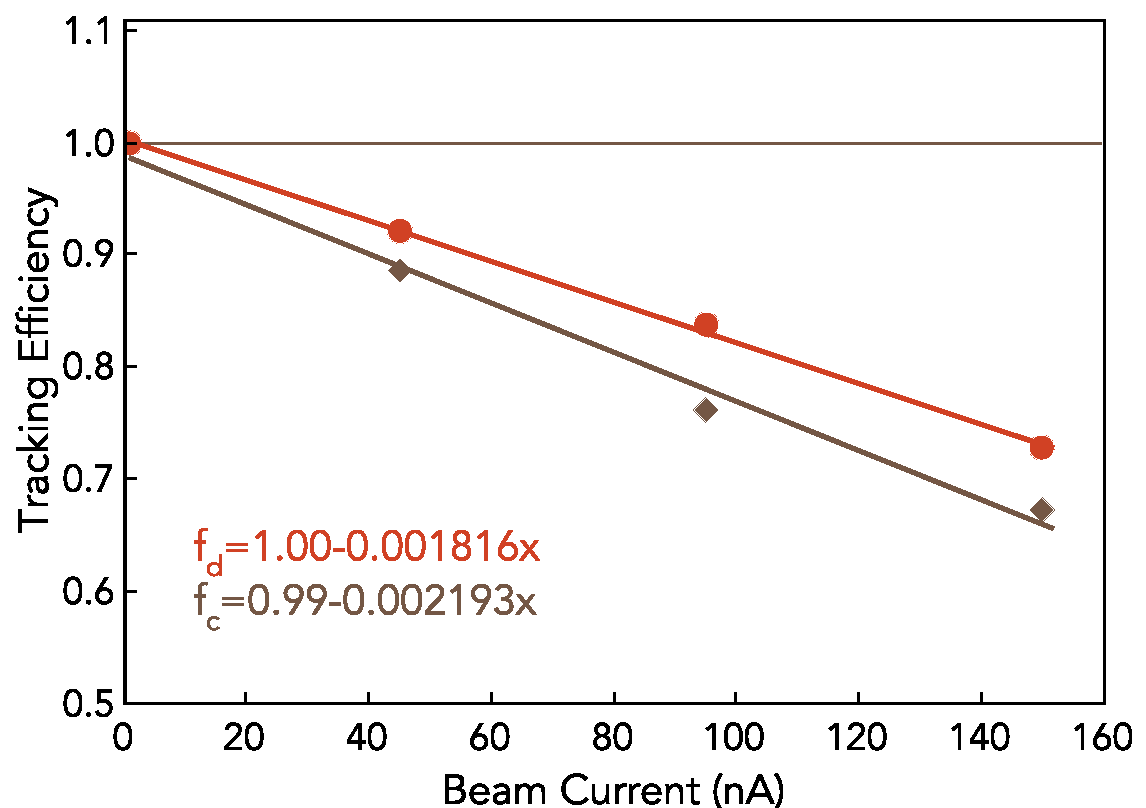
\includegraphics[width=3.1in]{images/figure_lscan_neg.pdf}
\caption {Tracking efficiency as a function of luminosity (beam current) for positively (a) and negatively (b) charged particle.  The efficiency is shown for
conventional algorithm running on background merged files (diamonds), and on files with merged background then de-noised with AI (circles).}
 \label{lscan::conv_dn}
 \end{center}
\end{figure}

As can be seen from the figure the number of reconstructed hadron-electron pairs relative to the number of reconstructed electrons is higher for the de-noised data sample compared to the raw data sample. This is due to an increased number of clusters reconstructed by the conventional clustering algorithm in the de-noised data samples. Detailed studies of cluster reconstruction efficiency are performed 
in our previously published article~\cite{Thomadakis:2022zcd}. 
The results show that the slope of the efficiency degradation as a function of the luminosity is significantly improved in the de-noised data sample. 
It is worth noting that the track reconstruction efficiency at 75 nA with de-noised data sample is the same as for the 
$45~nA$ when reconstructing raw data sample (without de-noising). This implies that the experiment can run effectively at $75~nA$, collecting data 
twice faster while maintaining the same track reconstruction efficiency, which will lead to higher experimental significance in measured observables. 

\subsection{Physics Impact}

The processed data was also evaluated to extract physics observables from both data samples to discern the impact on physics for the de-noising algorithm. As mentioned before, the data selected from the Pythia simulation was for the final state $H(e,e^\prime\pi^+\pi^-p)X$ containing exactly four charged particles. From this sample the missing mass distribution of $H(e,e^\prime\pi^+\pi^-)X$ is analyzed showing a peak around proton mass where the selected reaction is inclusive $\rho$ meson production and some background (above proton mass) where other reactions  are present (with missing neutral particles).

\begin{figure}[!h]
\begin{center}
 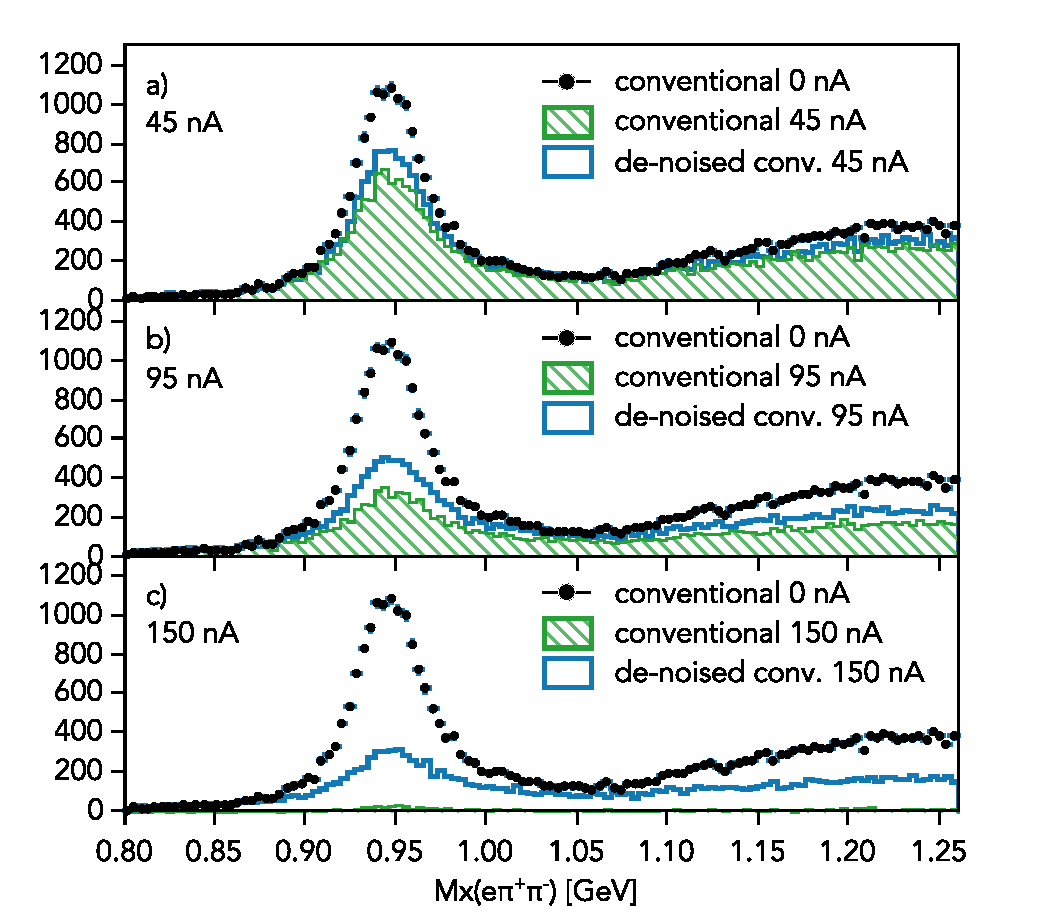
\includegraphics[height=3.1in]{images/plots_mxepipi_dn_ns.pdf}
   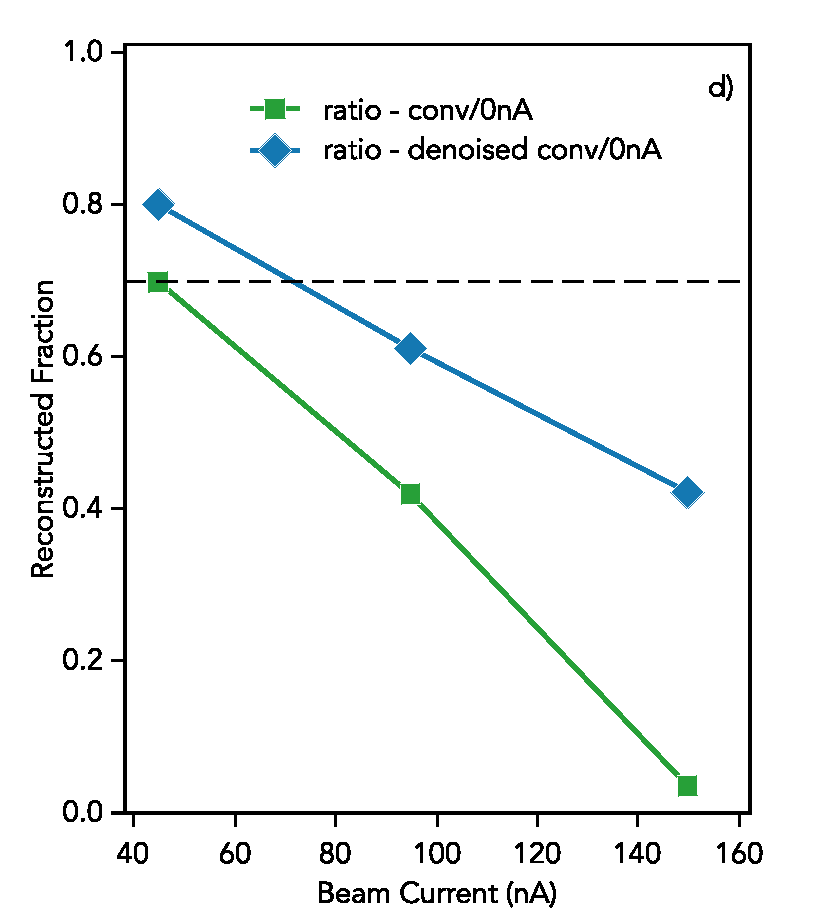
\includegraphics[height=3.1in]{images/graph_mxepipi_dn_ns.pdf}
\caption {
The de-noised data sample 
reconstructed with conventional algorithm (diamonds) for $45~nA$, $95~nA$ and $150~nA$. a), b) and c) reconstructed 
missing mass distributions for background merged data set reconstructed with conventional tracking (filled histogram) and
de-noised data sample reconstructed with conventional algorithm (solid line histogram).
d) The number of reconstructed protons from missing mass of $H(e \rightarrow e^\prime \pi^+\pi^-)X$ 
for background merged data set reconstructed with conventional tracking (squares) compared to de-noised data sample 
reconstructed with conventional algorithm (diamonds) for $45~nA$, $95~nA$ and $150~nA$.  }
 \label{physics::conv_dn}
 \end{center}
\end{figure}

In Figure~\ref{physics::conv_dn} the results of the analysis are shown, where the missing mass distribution $H(e,e^\prime\pi^+\pi^-)X$ is shown for different beam currents, in panels a), b) and c) the histograms show relative reconstructed distributions. The graph with points shows the missing mass reconstructed by the conventional tracking algorithm before any background is $0~nA$ for reference. The filled histogram shows the missing mass distribution reconstructed from background merged data with the conventional algorithm. The solid line histogram is the missing mass distribution reconstructed by a conventional algorithm after the background merged file is processed with a de-noising neural network to remove noise hits.
The summary of the number of protons in the missing mass distribution relative to the original (no background merged) distribution is presented in Figure~\ref{physics::conv_dn} d). It can be seen from the figure that the conventional algorithm reconstructs more tracks after de-noising the data. The number of reconstructed proton final states at $75nA$ from de-noised data is equal to the number of reconstructed final states at $45nA$ when using conventional track reconstruction algorithms.  Conducting experiments with higher incident beam current allows accumulating the necessary statistics for the proposed experiments in significantly less time, leading to huge savings in accelerator operations.

%\begin{figure}[!ht]
%\begin{center}
 %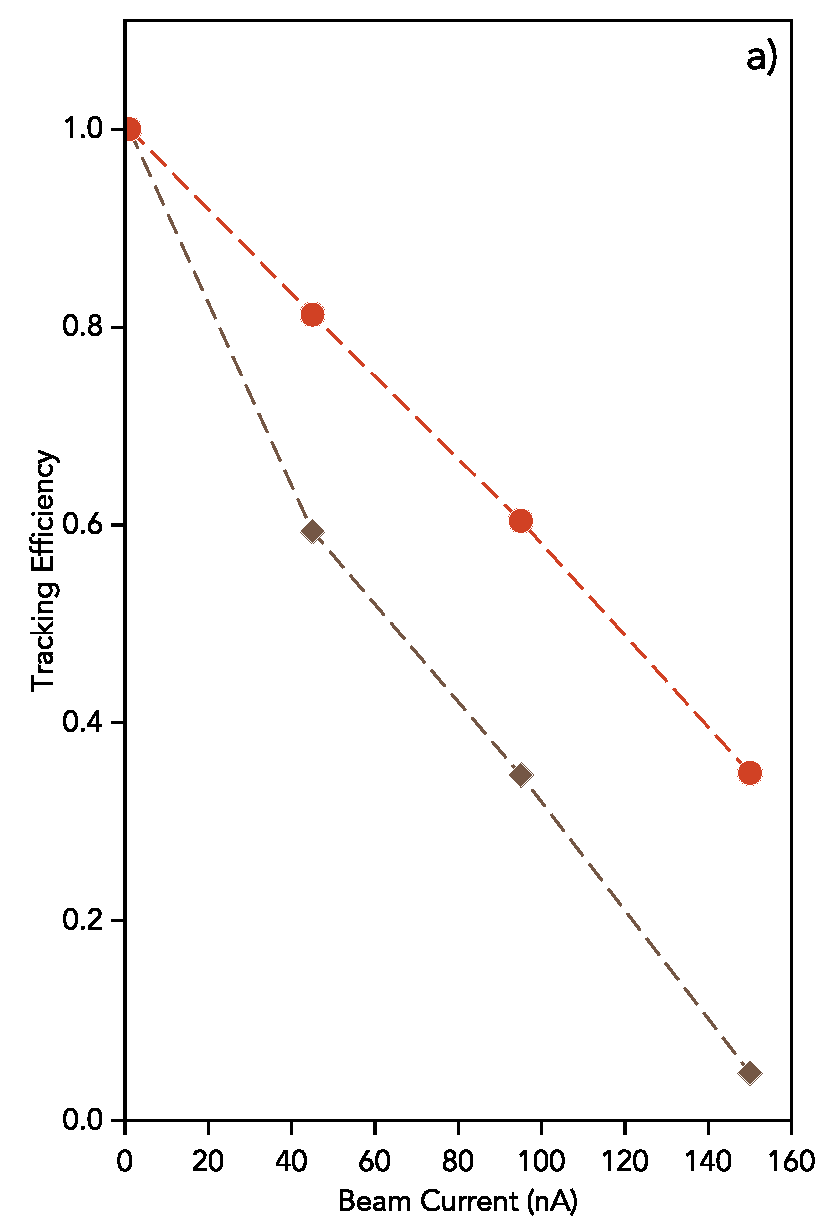
\includegraphics[width=3.1in]{images/figure_phys_scan.pdf}
 %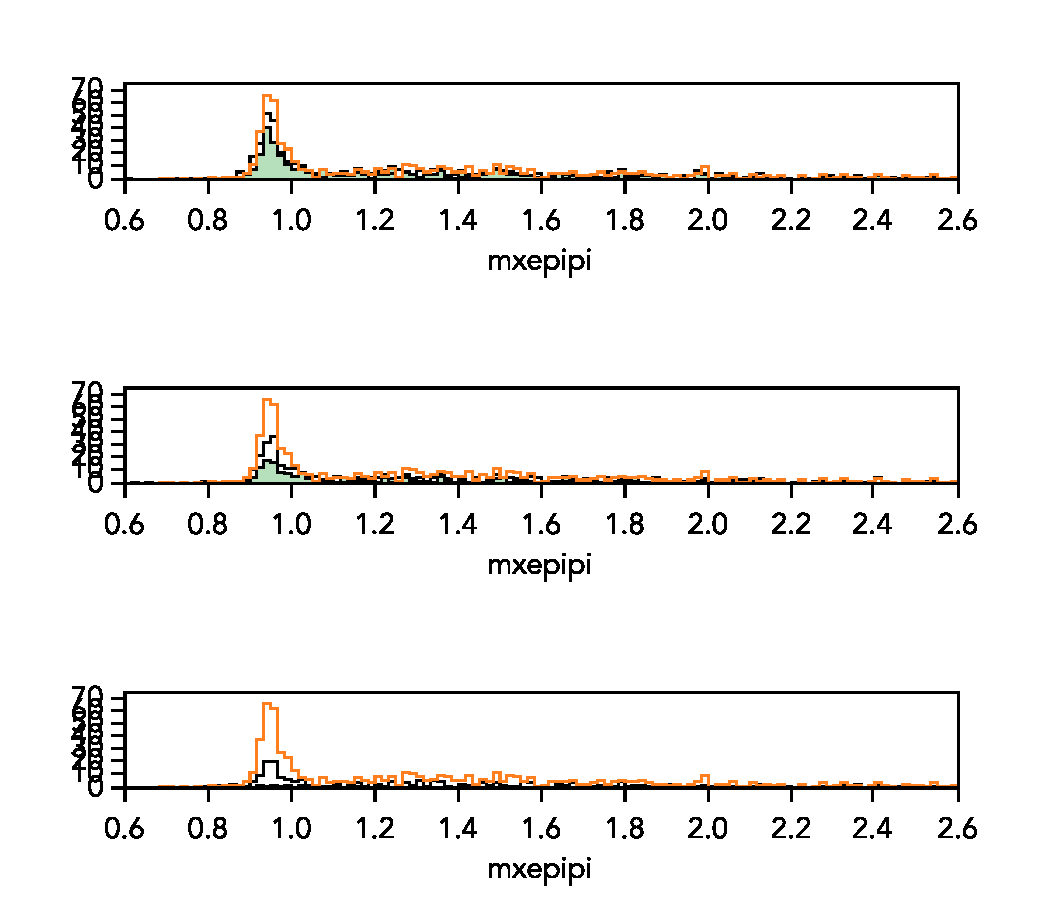
\includegraphics[width=2.5in]{images/figure_phys_conv_compare.pdf}
%\caption {Number of reconstructed protons from missing mass 
%of $H(e e^\prime \pi^+\pi^-)$ for background merged files for 
%$5~nA$, $45~nA$, $95~nA$ and $150~nA$ respectively.}
 %\label{physics::count_raw_dn}
 %\end{center}
%\end{figure}

%On Figure~\ref{physics::conv_dn} (a) the dependence is plotted for both data samples, where the points represent number of events under the proton peak normalized to the number of protons reconstructed by the tracking algorithm before background merging procedure (shown on Figure~\ref{physics::count_raw_dn} in the first column).
%It is evident from the figure that number of reconstructed protons in the de-noised data at $45~nA$ is $37\%$ larger, and the number of reconstructed protons at $95~nA$ in de-noised data sample is $2\%$ larger than in $45~nA$ background merged files. This result has significant implications on future experiments, since the data can be collected much fasted to reach the required statistical significance for given physics program while saving significant amount of money in accelerator operation costs.






\section{Data Analysis of De-Noising data with AI assistance}

The two data samples, background merged and de-noised, were also processed with new 
reconstruction software, which includes AI assisted track candidate identification~\cite{Gavalian:2022mlp}. The reconstruction software is designed to be able to process data in two parallel branches, where in one branch it reconstructs tracks with conventional algorithm where track candidates are identified by fitting all combinations of clusters forming a candidate and choosing candidates that pass the ``goodness'' of the fit criteria,  and on the second branch AI classifies track from the list of candidates crated from all combinations of clusters forming a track. This procedure is described in detail in~\cite{Gavalian:2022mlp}. Two samples were processed and comparison was made 
between conventional tacking algorithm from raw background merged files, and output of de-noised data sample with and without AI assisted tracking. 

\subsection{Luminosity dependence}

The track reconstruction efficiency was calculated for three samples using Eq.~\ref{eq::eff} for all three reconstructed data samples. The results are presented on Figure~\ref{lscan::conv_dn_ai}. It can be seen from the figure that using AI assisted tracking on de-noised data sample further improves reconstruction efficiency. The raw background merged data sample exhibits tracking efficiency decline of $0.23\%$ per nA, while the combination of de-noising and AI assisted tracking reduces this slope to $0.12\%$ (almost factor of 2), resulting in efficiency of $0.86\%$ at beam current $150~nA$ compared to $0.88\%$ at $45~nA$ beam current. 

\begin{figure}[!h]
\begin{center}
 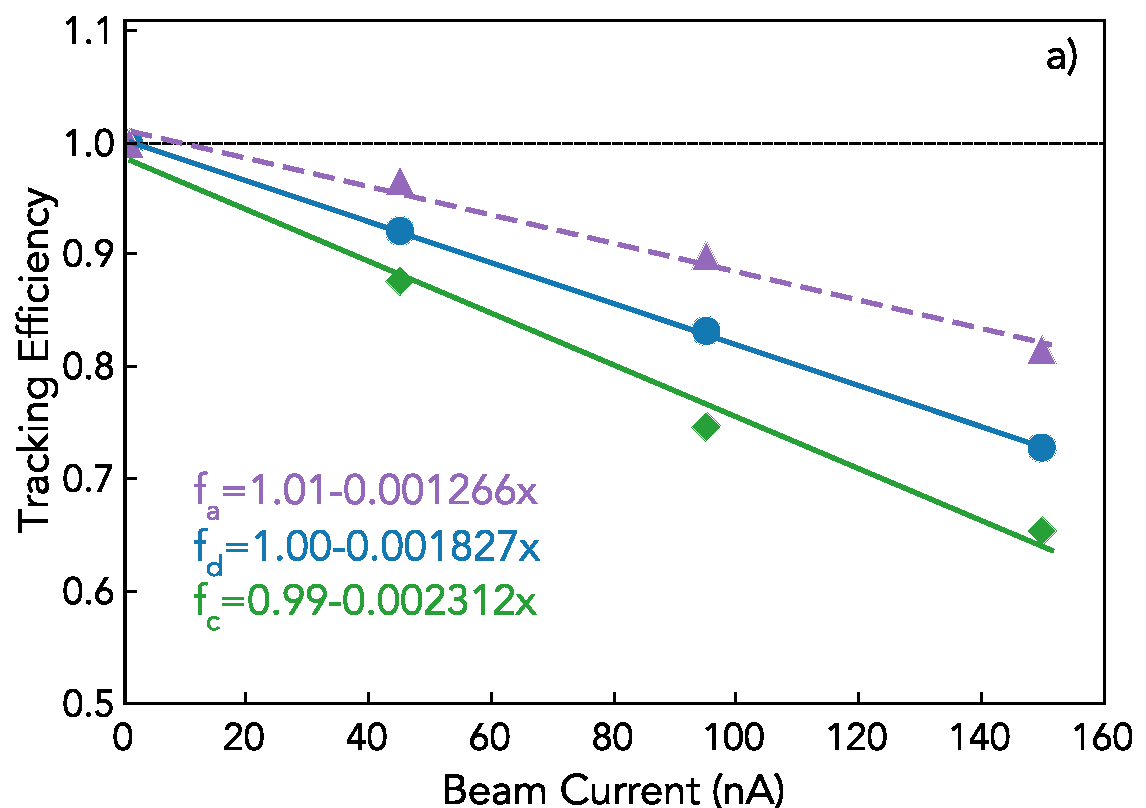
\includegraphics[width=3.1in]{images/figure_lscan_pos_ai.pdf}
 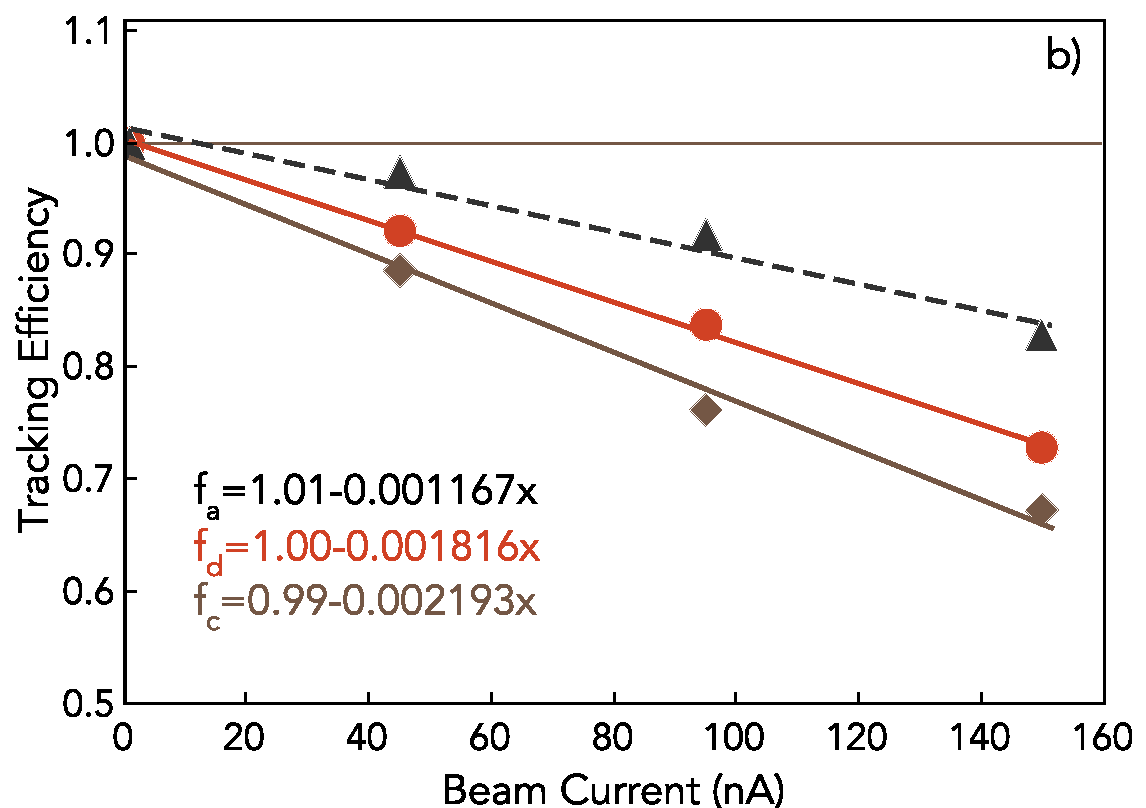
\includegraphics[width=3in]{images/figure_lscan_neg_ai.pdf}
\caption {Tracking efficiency as a function of luminosity (beam current) for positive (a) and negative particle (b).  The efficiency is shown for
conventional algorithm running on background merged files (diamonds), and on files with merged background then de-noised with AI (circles).}
 \label{lscan::conv_dn_ai}
 \end{center}
\end{figure}

This is significant improvement in tracking efficiency when using both AI assisted tracking with de-noising for beam current 3 times higher than current data collecting conditions.

\subsection{Physics Impact}

Further the physics impact was studied for de-noised data sample processed with AI assisted tracking. Same data sample was used in this studies with selected $H(e,e^-\pi^+\pi^-p)X$ event from Pythia simulations, and analyzed for
missing mass of $H(e,e^-\pi^+\pi^-)X$. The distributions of missing mass spectra are shown on Figure~\ref{physics::conv_dn_ai}.

\begin{figure}[!h]
\begin{center}
 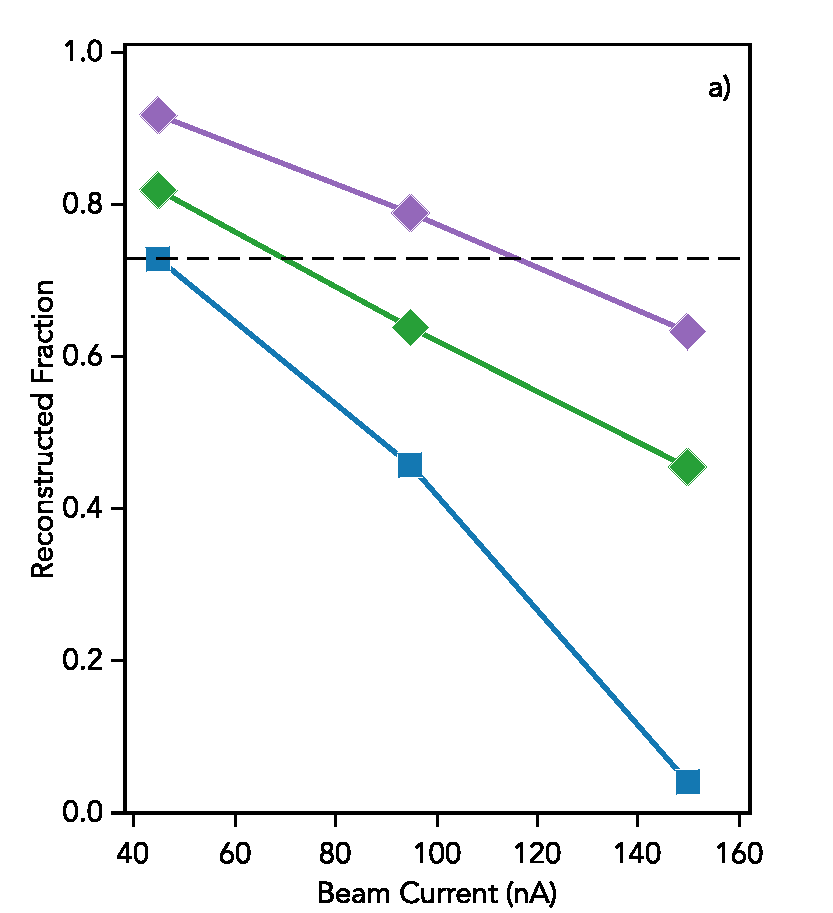
\includegraphics[height=2.8in]{images/graph_mxepipi_dn_ai.pdf}
 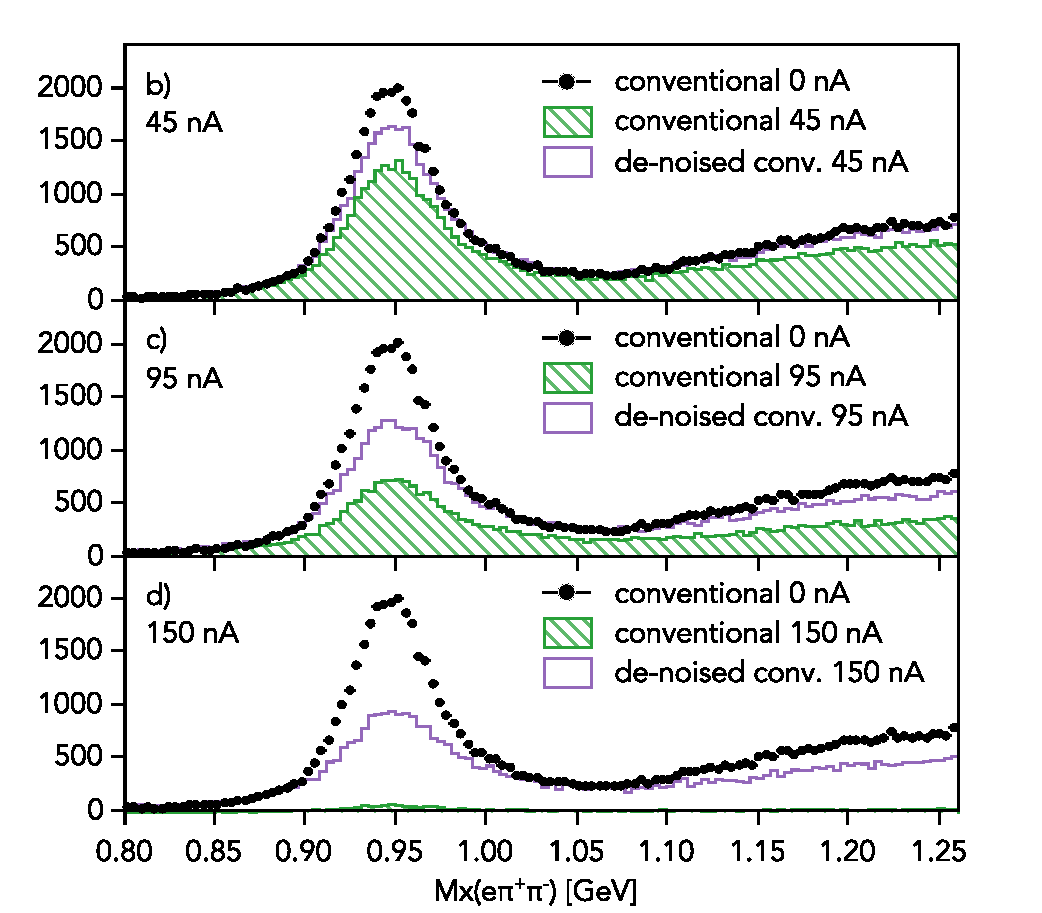
\includegraphics[height=2.8in]{images/plots_mxepipi_dn_ai.pdf}
\caption {Number of reconstructed protons from missing mass of $H(e \rightarrow e^\prime \pi^+\pi^-)$ for background 
merged files for  $5~nA$, $45~nA$, $95~nA$ and $150~nA$ respectively. The number of protons reconstructed by 
conventional algorithm after background merging is shown on the top row, and reconstruction after  de-noising drift 
chamber data on the bottom row.}
 \label{physics::conv_dn_ai}
 \end{center}
\end{figure}

The top row of plots shows missing mass distributions for different backgrounds reconstructed by conventional tracking algorithm. On the bottom row the distributions reconstructed from de-noised data sample are shown, with overlaid histograms (red) of AI assisted reconstruction. On Figure~\ref{physics::conv_dn_ai} a) the summarized analysis of missing mass distributions are shown where number of reconstructed protons are plotted for all three reconstruction scenarios. It is evident that adding AI assistance for track classification further improves physics outcome from data processing. It can be seen that for $95~nA$ data sample, the number of reconstructed protons with de-noising and AI assisted tracking is $14\%$ higher than number of protons from background merged file reconstructed using conventional (no AI involved) code.

\begin{table}
\begin{tabular}
Stats & Conventional & De-noised & De-noised + AI assisted \\
# nucleaons (45 nA)  & 27225 &  30576 & 34277 \\
# nucleaons (95 nA)  & 17125 & 23845 & 29428 \\
# nucleaons (150 nA) &  1576 & 17018 & 23601 \\
\hline
\hline
ratio to conventional 45nA & 1.0 & 1.12 & 1.26 \\
ratio to conventional 95nA & 1.0 & 1.39 & 1.72 \\
ratio to conventional 95nA & 1.0 & 10.80 & 14.97 \\
\end{tabular}
\caption{}
 \label{table:summary}
\end{table}






%\section{Analysis of experimental data}

We have verified that de-noising of background merged files significantly improves the track reconstruction efficiency.
It was shown that using AI assisted version of reconstruction software further improved the number of particles reconstructed for given reaction. 
The further checks experimental data collected with $45~nA$ incident beam energy was processed using de-noising software and then was processed with CLAS12 data reconstruction program. The same reaction $H(e,e^\prime\pi^+\pi^-)X$ was selected (for consistency) from experimental data and missing mass distributions were plotted for raw data, de-noised data reconstructed with conventional tracking algorithm and de-noised data reconstructed with AI assisted tracking algorithm.
The results are shown on Figure~\ref{denoise:exp_data}


\begin{figure}[!h]
\begin{center}
 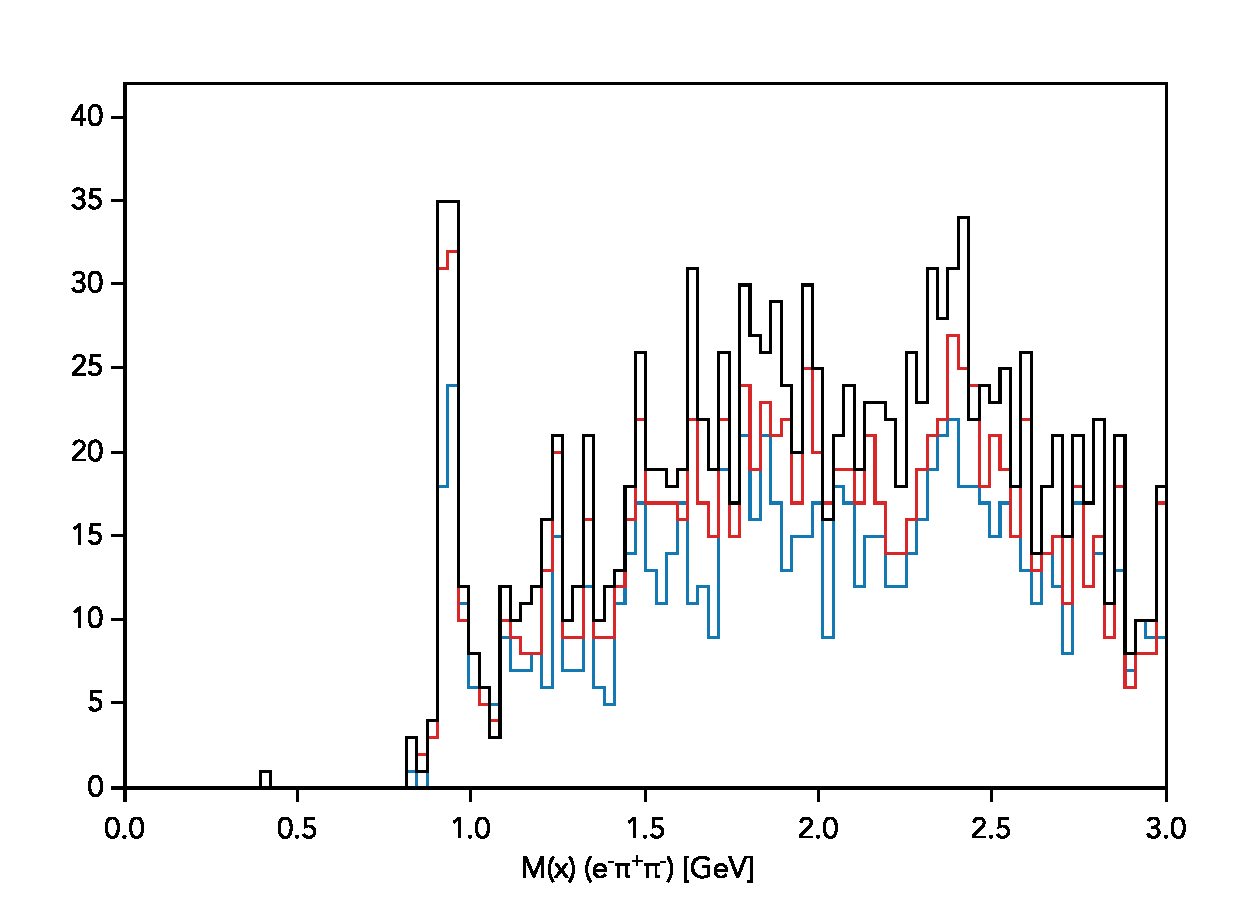
\includegraphics[width=3.1in]{images/figure_denoise_expdata.pdf}
\caption {Tracking efficiency as a function of luminosity (beam current) for positive (a) and negative particle (b).  The efficiency is shown for
conventional algorithm running on background merged files (diamonds), and on files with merged background then de-noised with AI (circles).}
 \label{denoise:exp_data}
 \end{center}
\end{figure}


\begin{table}[!h]
\begin{center}
\begin{tabular}{lccc}
Method & protons count & ratio &  MC ratio \\
\hline
Conventional & 41 & 1.00 & 1.00 \\
De-Noised & 59 & 1.43 & 1.37 \\
De-Noised with AI assisted & 70 & 1.71 &1.65 \\
\hline
\end{tabular}
\end{center}
\end{table}



%\section{Analysis of Track Reconstruction with AI}

After implementing the track identification service in the CLAS12 reconstruction software, the outputs
from the conventional tracking algorithm and AI-assisted tracking algorithm were analyzed
event by event to ascertain improvements of tracking. 
 
 \subsection{Particle Reconstruction efficiency}
 
 The Neural Network for track classification was trained on experimental data after it was processed with conventional tracking 
 reconstruction. Tracks that have ``good'' fit quality and were tracked back to the target were used as training samples for both 
 the MLP classifier and Auto-Encoder corruption-recovery network. For more detailed analysis of tracking reconstruction performance with and without assistance from artificial intelligence we processed one run at nominal luminosity (45 nA) to compare performances.
 
 %The efficiency of track reconstruction was obtained for separate track topologies (6 super-layer and 5 super-layer).
 \begin{figure}[!ht]
\begin{center}
% 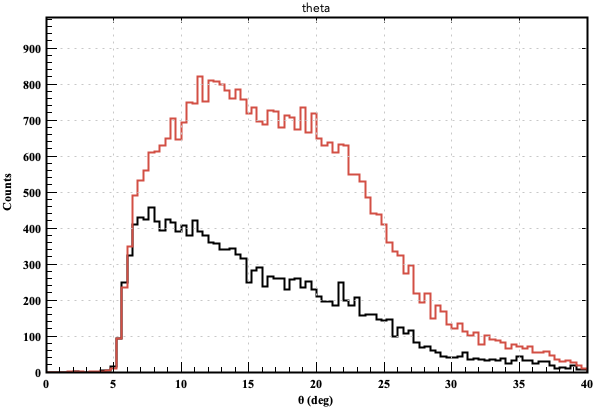
\includegraphics[width=2.0in]{images/pos_theta_5SL.png}
  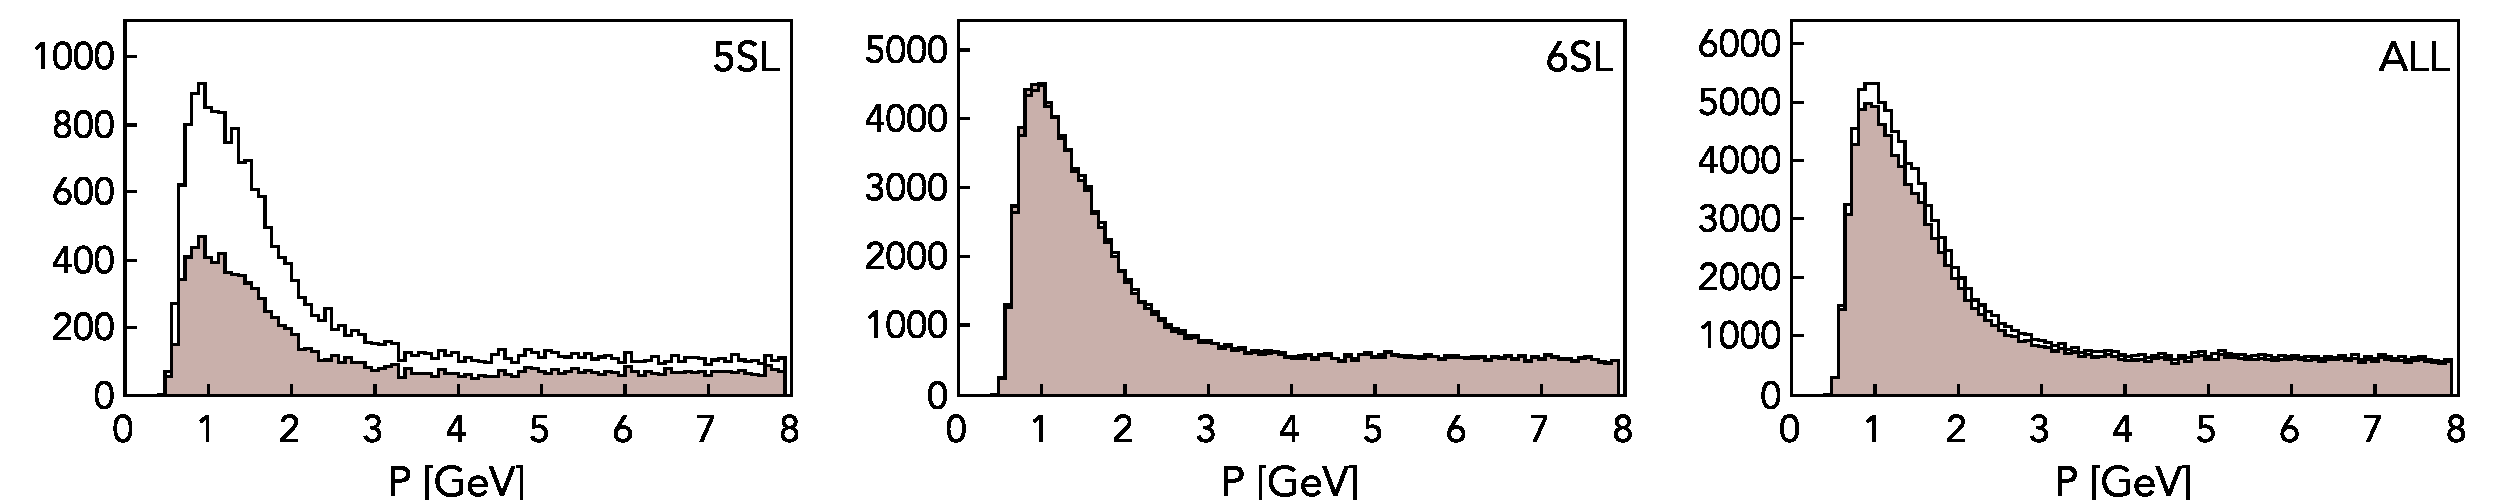
\includegraphics[width=6.5in]{images/figure_p.pdf}
  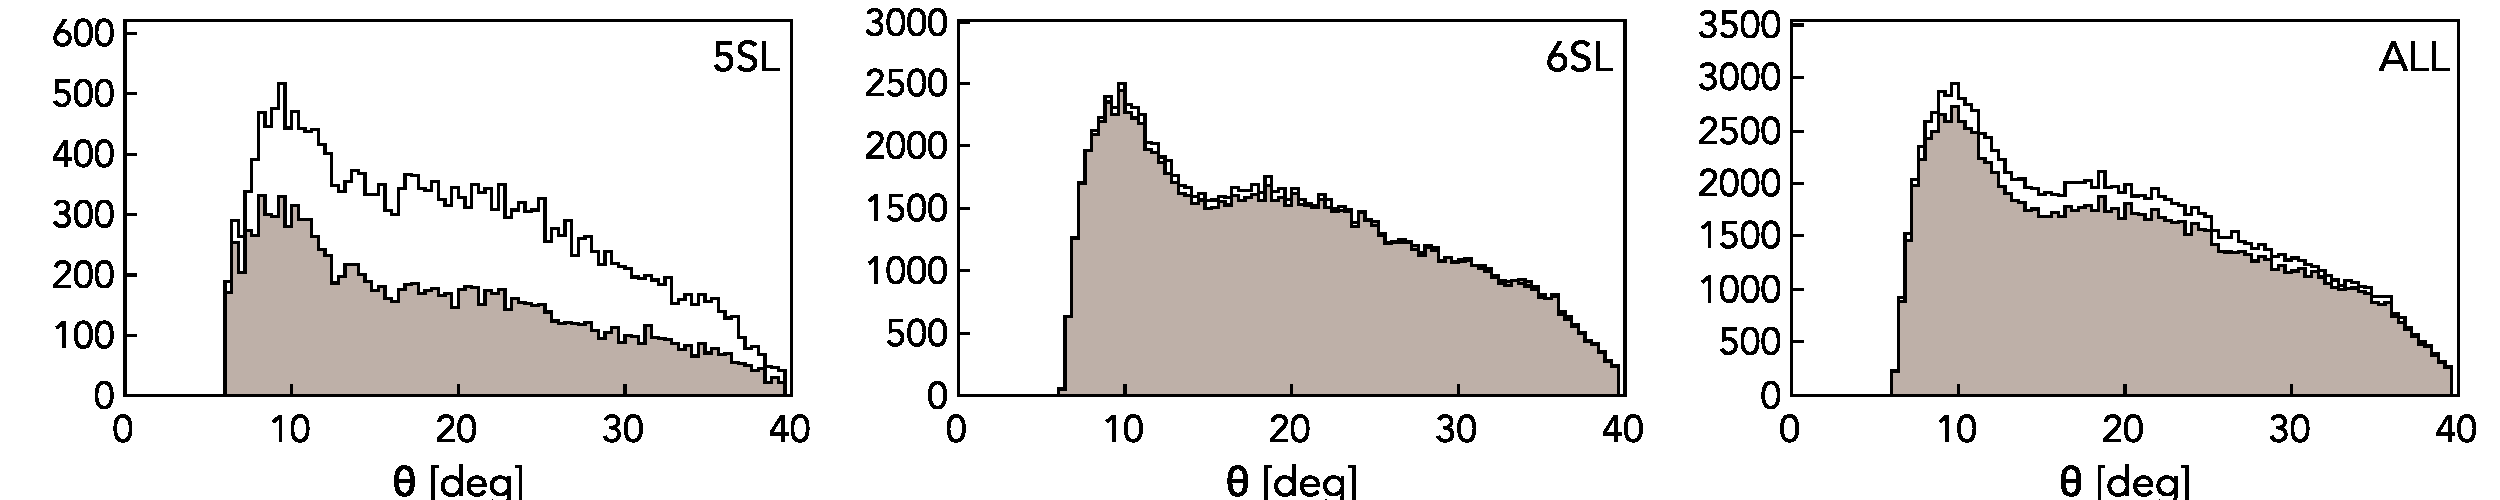
\includegraphics[width=6.5in]{images/figure_theta.pdf}
    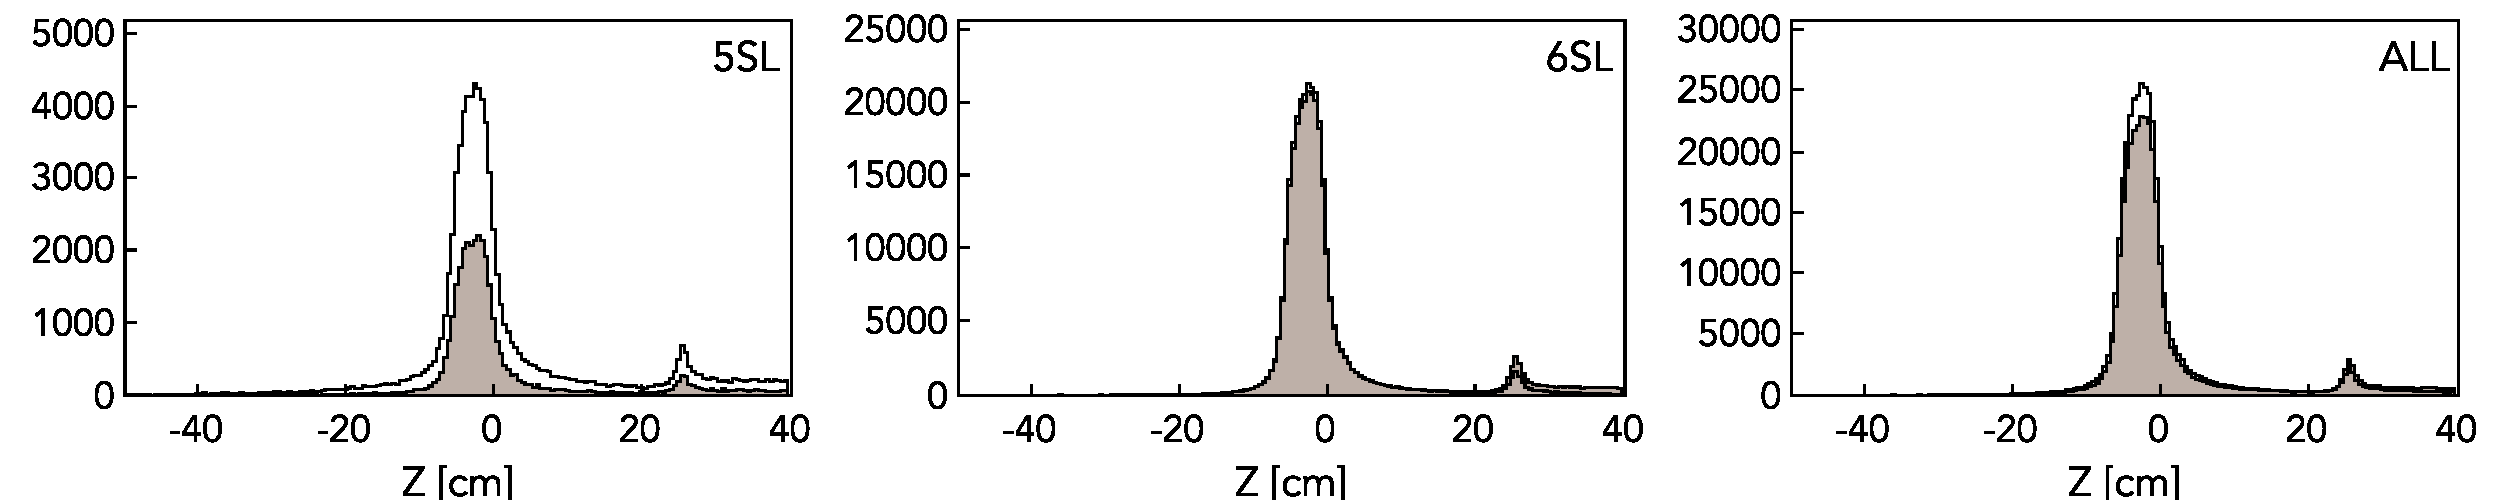
\includegraphics[width=6.5in]{images/figure_vz.pdf}
\caption { Comparison of number of tracks reconstructed with the conventional algorithm (filled histograms) vs AI-assisted tracking code (open black outline histograms) as a function of momentum, polar angle and particle interaction vertex. The comparison is shown for 5 super-layer, 6 super-layer tracks (left two columns), and the total number (right column).}
 \label{track:efficiency}
 \end{center}
\end{figure}

The results are shown on Figure~\ref{track:efficiency}, where dependence of number of reconstructed negatively charged 
 tracks are shown as a function of particle momentum (top row), polar angle in laboratory frame (bottom row) and interaction
 vertex (middle row). The reconstructed distributions from conventional tracking are plotted with filled histograms and the
 tracks reconstructed using assistance from AI are plotted with solid lines. As can be seen from the figure, there is a large gain 
 in the number of reconstructed tracks with the 5 super-layer configuration compared to full 6 super-layer tracks. Typically for nominal 
 45 nA experimental data increase in track efficiency for 6 super-layers tracks averages about $3\%-6\%$, while for 5 super-layer
 tracks the increase is in the order of $70\%-120\%$. In normal data reconstruction, tracks that are identified with 5 super-layers
 usually comprise about $10\%$ of all reconstructed tracks, and a significant increase in identification of such tracks leads to 
 overall tracking efficiency increase of $12\%-15\%$. 
 
 \begin{table}[!h]
 \begin{center}
 \begin{tabular}{|l|c|c|c|c|}
 \hline
 Track Configuration & Conventional & AI Assisted & Gain & Relative \\
 \hline
 \hline
 6 Super-Layer & 242,145 & 256,175 & 14030 & 1.0579 \\
 5 Super-Layer & 24,155 & 52,839 & 28684 & 2.1875 \\
 All & 267,339 & 309,058 & 51719 & 1.1561 \\
 \hline
 \end{tabular}
 \end{center}
 \caption{Summary of reconstructed tracks and gain with assistance from Artificial Intelligence.}
 \label{tbl:summary}
 \end{table}
 
The comparison of 5 and 6-segment track statistics and their relative gain is summarized in Table~\ref{tbl:summary}.
As can be seen from the table the gain in only 6-segment tracks is about $5.7\%$ but with significant gain in 5 super-layer tracks 
the overall gain in reconstructed tracks elevates to $>15\%$. These results are intuitive since track candidates composed of 5
super-layers with the same number of clusters in each super-layer are significantly higher than 6 super-layer track candidates, and 
in our tests AI performs better in choosing the right combination with increasing combinatorics.
 
\subsection{Luminosity Dependence}

Track reconstruction efficiency increased with AI-assisted tracking, since AI can better identify tracks
from a pool of candidates. One would expect that if the number of combinations decrease the efficiency 
of the conventional track selection algorithm should approach the efficiency of AI-assisted track identification.
Similarly, when the number of combinations increases the advantage of AI over the conventional algorithm should
increase. Based on this we expect AI to perform better in higher background settings. To evaluate AI-assisted
tracking efficiency dependence on background we analyzed several different runs that were taken in different 
conditions (i.e. beam current) ranging from $5~nA$ to $70~nA$. To measure tracking efficiency we first calculated
the number of electrons ($N_e$) detected in the data sample analyzed (typically one run) and then the number of positive and negative
 hadrons that were detected with the electron inclusively ($N_{h^+e}$ and $N_{h^-e}$ respectively).

Then the efficiency for the data set was calculated as:

\begin{equation}
L_t^+ = \frac{N_{h^+e}}{N_e} , L_t^- = \frac{N_{h^-e}}{N_e} 
\end{equation}

where $L_t^+$ is the efficiency of positive particles and $L_t^-$ is the efficiency of negatively charged particles respectively. 
In order to estimate the charged particle reconstruction efficiency as a function of the beam current, the multiplicity, $L_t^{+/-}$, is fitted with a linear function:
\begin{equation}
L_t^{+/-} = a + c\times I 
\end{equation}

Here $a$ and $c$ are the fit parameters and $I$ is the beam current. Then it was assumed that the reconstruction efficiency, $E=1$ at $I=0$ nA:

\begin{equation}
E^{+/-} = 1 + b \times I 
\end{equation}

with $b=\frac{c}{a}$. The slope parameter b is the rate of the reconstruction inefficiency as a function of the beam current \cite{Stepanyan:2020bg}.
%The all points were 
%fitted with linear function $L=a+bx$, where $a$ is the intercept 
 
 \begin{figure}[!ht]
\begin{center}
 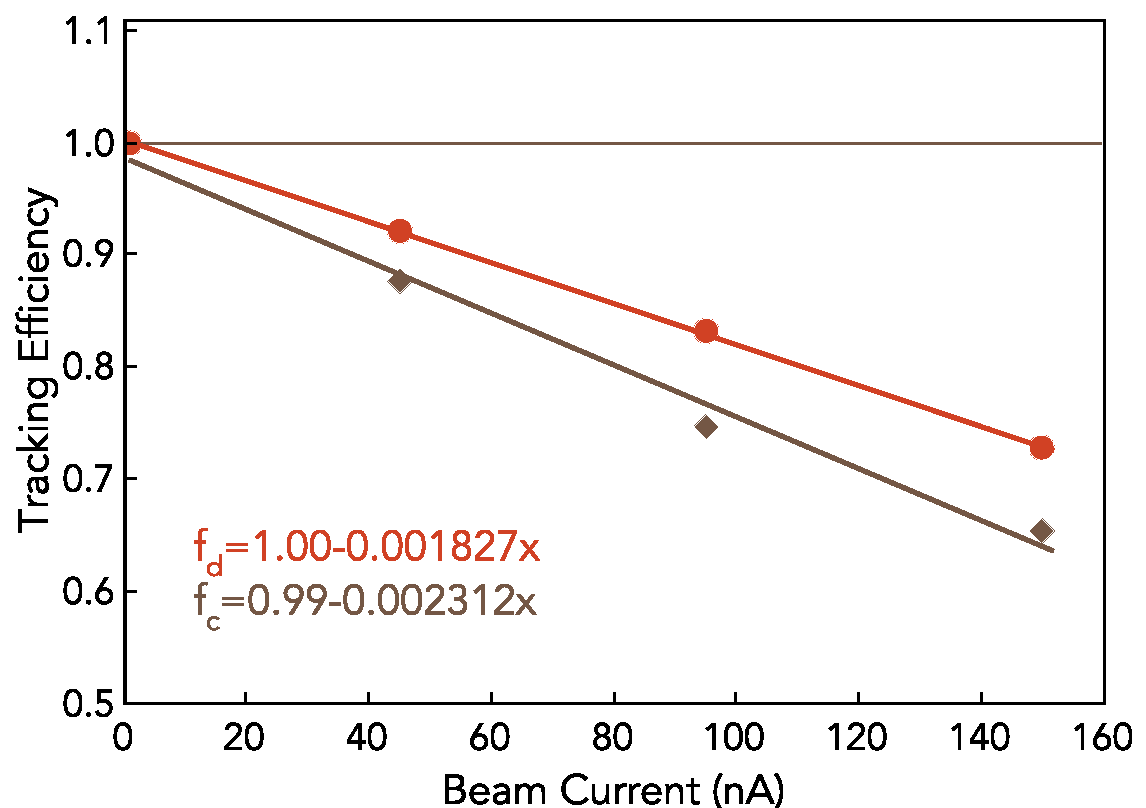
\includegraphics[width=3.0in]{images/figure_lscan_pos.pdf}
 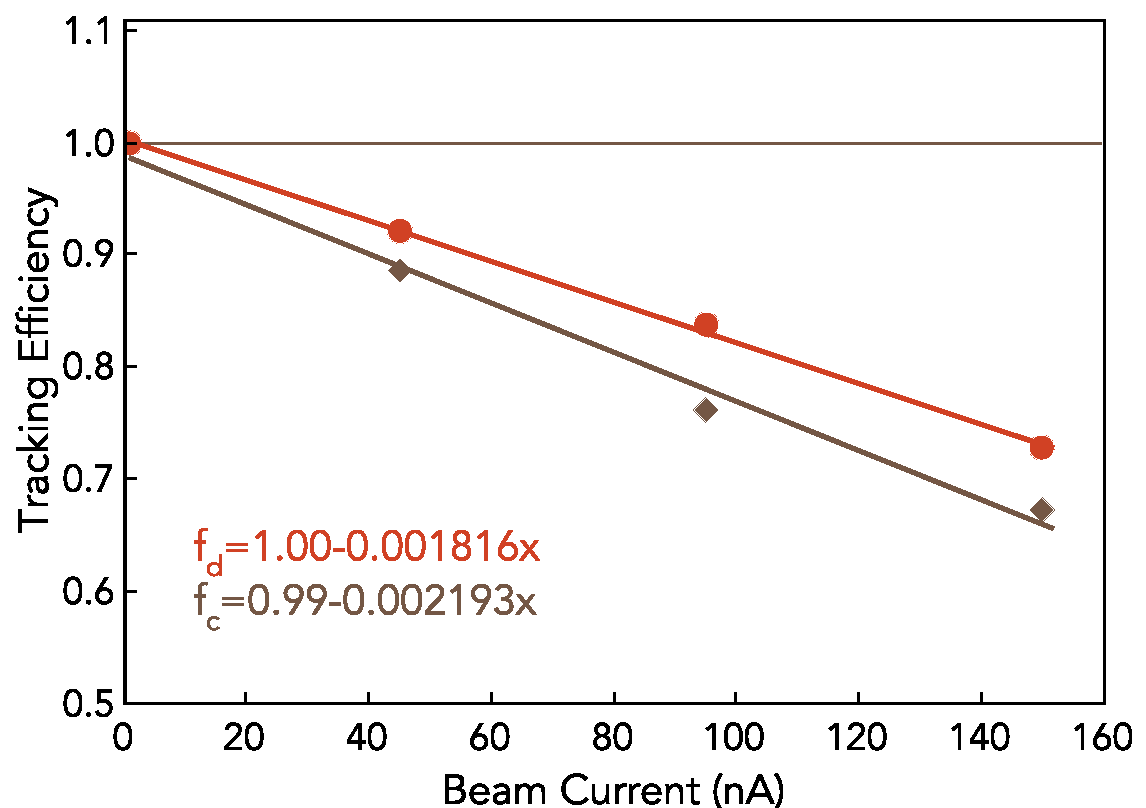
\includegraphics[width=3.0in]{images/figure_lscan_neg.pdf}
\caption {Tracking efficiency for positively and negatively charged particles as a function of beam current (luminosity).  Conventional algorithm 
track reconstruction efficiency (diamonds) is compared to AI-assisted track reconstruction efficiency (circles). }
 \label{lumi:scan}
 \end{center}
\end{figure}

The comparison of tracking efficiency as a function of beam current (luminosity) can be seen on Figure~\ref{lumi:scan} where $E^{+/-}$ are shown for positively and negatively charged particles separately. As can be seen from the figure, AI-assisted tracking performs significantly better for any given luminosity (beam current) and the decrease of efficiency is much slower as a function of luminosity, $0.22\%$ per nA versus $0.40\%$ per nA for conventional tracking. This is expected and consistent with the assumption that with increased combinatorial background (increased number of track candidates to consider), AI performs better in choosing the best track candidate. We established that AI-assisted
tracking leads to more tracks reconstructed for any given beam current setting. The next thing to check is what is the impact of increased track reconstruction efficiency on physics analysis.
% and if there is increase in physics outcome for the CLAS12 experimental setup.

\subsection{Physics Impact}

To measure practical implications of track reconstruction efficiency improvement on physics outcome we analyzed 
two event topologies with two particle and three particles in the final state respectively. The data for analysis were 
taken with $10.5~GeV$ electron beam incident on $20~cm$ liquid hydrogen target, with a beam current of $45~nA$
(typical for CLAS12 experimental running). We selected events where an electron was detected in the forward detector, and 
then isolated events where there was an additional negatively charged pion ($\pi^-$) along with an electron and no other 
charged particle. The second topology required two pions along with electron, one positively charged and one 
negatively charged. The two chosen topologies are denoted by $H(e,e'\pi^-X)$ and $H(e,e'\pi^+\pi^-X)$. In both cases 
there is a visible peak of a missing proton that we can use to measure the impact of efficiency on physics outcome. 

 \begin{figure}[!ht]
\begin{center}
 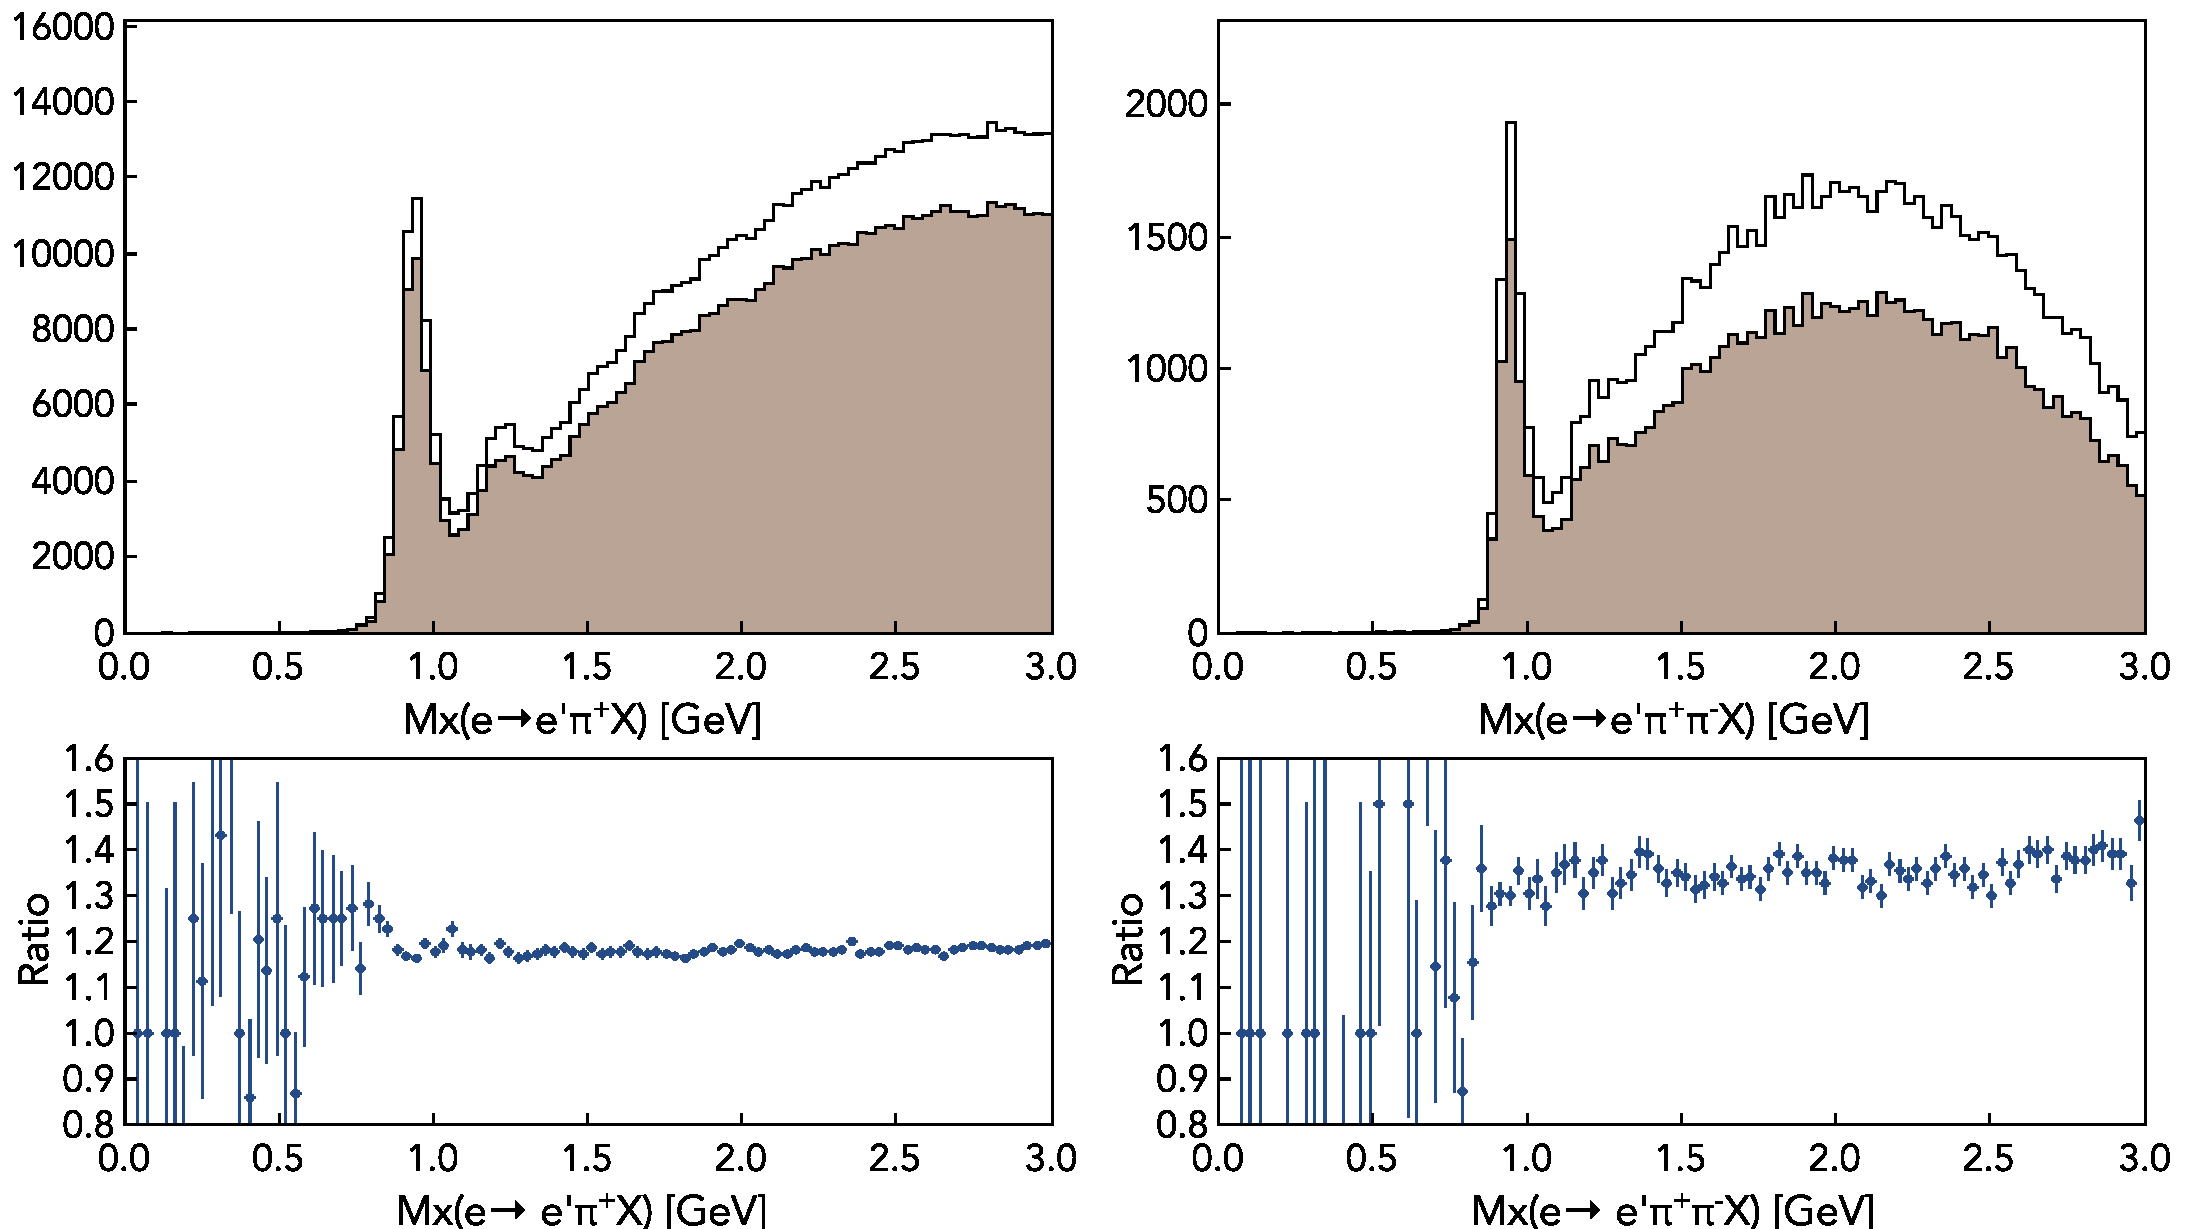
\includegraphics[width=6.0in]{images/physics_scan.pdf}
\caption {Reconstructed missing mass distribution for $H(e,e'\pi^-X)$ and $H(e,e'\pi^+\pi^-X)$ reactions (top row) using the conventional track reconstruction algorithm (filled histogram) and  AI-assisted track reconstruction (black line histogram). The ratios of the two histograms are shown on the bottom row. }
 \label{physics:outcome}
 \end{center}
\end{figure}

The distributions of missing mass for both final state topologies are shown on Figure~\ref{physics:outcome}, where the plots 
on the top row are missing mass of $H(e,e'\pi^-X)$ and $H(e,e'\pi^+\pi^-X)$, where the filled histogram is calculated from 
particles reconstructed by the conventional tracking algorithm, and the histogram with black outline are the same distributions 
calculated from particles that were reconstructed using suggestion from Artificial Intelligence. As can be seen from the figure, 
there is significant increase in the number of events under the missing proton peak (at mass value $0.938~MeV$) for AI assisted
tracking. The ratios of the two histograms (AI-assisted divided by conventional) can be seen on the bottom row of 
Figure~\ref{physics:outcome}. As can be seen from the figure the increase in statistics is uniform over the whole range of the 
missing mass indicating no systematic abnormalities for AI-assisted tracking. The ratio also indicates that there is an increase 
for the number of events under the peak for proton, about $15\%$ for $H(e,e'\pi^-X)$ final state and $30-35\%$ for the $H(e,e'\pi^+\pi^-X)$
final state. Further studies show that improvements in statistics are larger for higher luminosity (incident beam current), which is consistent with our studies of increased efficiency of single particle reconstruction.
%Further studies show that increase in statistics for different final states increase with increase of beam current (luminosity) 
%which is consistent with our studies of increased efficiency of single particle reconstruction. 


\section{Summary}

In this paper we investigated results of analysis of experimental data from CLAS12 detector reconstructed with assistance of Artificial Intelligence
to identify tracks from the hits in drift chambers. This work is based on two neural networks developed to classify track candidates from
given cluster combinations \cite{Gavalian:2020oxg} and to identify missing cluster positions in tracks that do not have complete 6 cluster configuration \cite{Gavalian:2020xmc}. After implementing these networks into the CLAS12 reconstruction workflow, the AI was able to identify ``good'' track candidates 
and pass them to the tracking code to be analyzed parallel to conventional algorithm that chooses``good'' track candidates iteratively considering all possible combinations. 
Our studies showed that AI-assisted tracking performs better than conventional track identification algorithm, and leads to track reconstruction efficiency increase of $15\%$ for nominal experimental running conditions (beam current 45 nA). The AI also performs better with increasing background (i.e. with increased incident beam current) and improves the efficiency loss from $0.44\%$ per nA to $0.24\%$ per nA.
This increased track reconstruction (identification) efficiency directly impacts the outcome of physics analysis where it increases statistics 
for physics reactions for $15\%-35\%$ depending on how many particles are detected in the final state and the topology of the reaction. This has significant implication on experimental running conditions since with increased efficiency the required statistical significance of the experiment can be reached in a shorter time by running at higher beam current (luminosity). Already collected experimental data can be re-processed with the AI-assisted tracking
code which can increase the statistics for analyzed data up to $35\%$. Both, future experiments and already completed ones will benefit 
from this novel development.

Another important outcome of this development was a reduction in data processing times. Since track candidates were identified by AI, there were fewer marginal quality tracks picked to be analyzed and then later dropped due to non-convergence of Kalman filter, leading to tracking code speedup  of $35\%$.

Overall we identified that AI assistance in tracking codes is a good approach, and leads to improvements in code speed and 
efficiency of track reconstruction. Another important aspect of using AI is that is leads to a very small and simple codebase, comprised of composing track candidates and feeding them to the neural networks, and what's also important is that it keeps improving with constant training on new data.
We intend to continue this development in extending the approach to other tracking detectors of the CLAS12, and possibly try to adapt  our approach for other experimental detector setups at Jefferson Lab.

Given the increase in track reconstruction and significant increase in physics statistics for nominal data taking conditions at $45~nA$ we estimated savings of  $\$4.2$M USD. The calculation was done using publicly available budget for operating CEBAF~\cite{CEBAF:oper} adjusted for inflation~\cite{GoogleDotCom}. The calculated budget of ~\$$48$M for all four experimental halls annually means $\approx \$12$M operating budget for CLAS12 experiments, and with $\approx 35\%$ increase in statistics leads to reported savings.




\section{Discussion}

So it goes.



\newpage

\section{Acknowledgments}

This material is based upon work supported by the U.S. Department of Energy, Office of Science,
Office of Nuclear Physics under contract DE-AC05-06OR23177, and NSF grant no. CCF-1439079 and
the Richard T. Cheng Endowment. This work was performed using the Turing and Wahab computing
clusters at Old Dominion University.
 
\newpage
\bibliography{references}
\bibliographystyle{ieeetr}

\end{document}
